%\author{\href{https://bit.ly/lorentztransformation}{Google AI studio prompt}\\ \small \emph{Derivado de los Postulados de la Relatividad Especial}}

\documentclass[11pt,a4paper]{article}

% --- PAQUETES ---
\usepackage[margin=1in]{geometry} % Establecer márgenes de página
\usepackage{amsmath}              % Para entornos matemáticos avanzados como aligned, pmatrix, boxed
\usepackage{amssymb}              % Para símbolos matemáticos adicionales
\usepackage{graphicx}             % Para incluir gráficos
\usepackage{cancel}    
\usepackage[dvipsnames]{xcolor}
\usepackage{hyperref}             % Para hipervínculos y metadatos del PDF
\hypersetup{
    colorlinks=true,
    linkcolor=blue,
    filecolor=magenta,      
    urlcolor=cyan,
    pdftitle={Derivación de las Transformaciones de Lorentz},
    pdfauthor={Asistente de IA},
    bookmarks=true,
    pdfpagemode=UseOutlines,
}
\usepackage{enumitem}
\usepackage{tikz}
\renewcommand{\arraystretch}{1.9}

% --- INFORMACIÓN DEL TÍTULO ---
\title{Una Derivación Completa de las Transformaciones de Lorentz \\ y su Interpretación Geométrica}
\author{\href{https://bit.ly/lorentztransformation}{Google AI studio prompt}\\ \small \emph{Derivado de los Postulados de la Relatividad Especial}}
\date{\today}

% --- INICIO DEL DOCUMENTO ---
\begin{document}

\maketitle
\tableofcontents


\begin{abstract}
Este documento proporciona una derivación detallada y paso a paso de las transformaciones de Lorentz, fundamentada en los postulados de la Relatividad Especial. Luego, extiende esta derivación para explorar la estructura geométrica más profunda de las transformaciones, introduciendo los conceptos de rapidez y el formalismo matricial. Finalmente, demuestra cómo un impulso de Lorentz (boost) puede ser visto formalmente como una rotación en un espaciotiempo complejo a través de una rotación de Wick.
\end{abstract}

\section{Introducción}

Las transformaciones de Lorentz son la piedra angular de la teoría de la Relatividad Especial de Einstein. Relacionan las coordenadas de espacio y tiempo de un evento según lo medido por dos observadores en diferentes sistemas de referencia inerciales. Reemplazan a las antiguas transformaciones de Galileo, que son inconsistentes con la constancia observada de la velocidad de la luz.

La derivación se basa en dos postulados fundamentales de la Relatividad Especial:
\begin{enumerate}
    \item \textbf{El Principio de Relatividad:} Las leyes de la física son las mismas en todos los sistemas de referencia inerciales.
    \item \textbf{La Constancia de la Velocidad de la Luz:} La velocidad de la luz en el vacío, denotada por $c$, es la misma para todos los observadores inerciales, independientemente del movimiento de la fuente de luz o del observador.
\end{enumerate}

El segundo principio puede ser cambiado simplemente por la suposición de que el espacio y el tiempo deben ser homogéneos e isotrópicos, ver \url{https://arxiv.org/pdf/gr-qc/0107091}

La motivación de la relatividad especial surge de la necesidad de usar el primer postulado para la interacción electromagnética. Aunque dicho postulado es evidente en sistemas mecánicos, no es claro para la interacción electromagnética. De hecho, una partícula cargada en reposo sólo tiene asociado un campo eléctrico, mientras que una partícula moviéndose a velocidad constante relativa al observador en reposo, genera una corriente eléctrica que a su vez induce un campo magnético. Además, el campo eléctrico se deforma (las regiones de campo constante pasan de ser esféricas a elipsoidales). Cómo en última instancia los objetos de medida están hechos de partículas cargadas dentro de los átomos que la componen, es de esperarse

\section{Noción de transformaciones}

Un ejemplo de transformación es la de un montaje experimental en la cual se determina el movimiento de un cuerpo con respecto a los ejes $x$, $y$ correspondientes a los lados de la mesa ilustrado en la figura~\ref{fig:tabla} izquierda. Posteriormente se repite la medida con la mesa rotada un ángulo $\theta$ pero manteniendo la posición del montaje experimental sobre la misma, como se ilustra en la figura~\ref{fig:tabla} derecha. Es claro que la trayectoria del movimiento no depende del sistema de referencia.
\begin{figure}
  \centering
  \includegraphics[scale=0.4]{table}
  \includegraphics[scale=0.4]{tabletheta}
  \caption{Rotación de sistema de coordenadas}
  \label{fig:tabla}
\end{figure}




\begin{figure}
  \centering
  \includegraphics[scale=0.75]{so2}
  \caption{Rotación por ángulo $\theta$}
  \label{fig:so2}
\end{figure}



Considere un punto $(x,y)$ en sistema de referencia de dos dimensiones. Si cambiamos a un sistema de referencia rotado por un ángulo $\theta$, $(x',y')$, como se muestra en la figura~\ref{fig:so2}, podemos definir los dos triángulos rectángulos que se muestran en la figura y a partir de ellos obtener la transformación de los sistemas de referencia debido a la rotación
\begin{align}
  x'=&x\cos\theta+y\sin\theta \nonumber\\
  y'=&y\cos\theta-x\sin\theta\,.
\end{align}

% --- Inicio del código para insertar ---

% Para las ecuaciones matemáticas
\begin{align*}
    \boldsymbol{r} &= (x, y) \\
    \boldsymbol{r}' &= (x', y') \\[1em] % Añade un poco de espacio vertical
    r^2 = \boldsymbol{r} \cdot \boldsymbol{r} &= x^2 + y^2 \\
  {r'}^2 =  \boldsymbol{r}' \cdot \boldsymbol{r}' &= x'^2 + y'^2 = x^2 + y^2 = \boldsymbol{r} \cdot \boldsymbol{r}
\end{align*}

La demostración del último paso se hace a continuación.

% --- Inicio del código para insertar ---

\subsection*{Demostración de la Invariancia del Producto Escalar bajo Rotación}

El objetivo es demostrar que el módulo al cuadrado de un vector es el mismo después de una rotación de coordenadas. Es decir, probaremos que:
\[
\boldsymbol{r}' \cdot \boldsymbol{r}' = \boldsymbol{r} \cdot \boldsymbol{r} \quad \Leftrightarrow \quad x'^2 + y'^2 = x^2 + y^2
\]

\subsubsection*{Paso 1: Ecuaciones de Transformación por Rotación}
Las coordenadas $(x', y')$ en un sistema que ha sido rotado un ángulo $\theta$ en sentido antihorario se relacionan con las coordenadas originales $(x, y)$ mediante:
\begin{align*}
    x' &= x \cos\theta + y \sin\theta \\
    y' &= -x \sin\theta + y \cos\theta
\end{align*}

\subsubsection*{Paso 2: Sustitución y Expansión Algebraica}
Sustituimos estas transformaciones en la expresión para el módulo al cuadrado en el sistema rotado, $\boldsymbol{r}' \cdot \boldsymbol{r}' = x'^2 + y'^2$.

\begin{align*}
    x'^2 + y'^2 &= (x \cos\theta + y \sin\theta)^2 + (-x \sin\theta + y \cos\theta)^2 \\[1em]
    % Expandiendo los binomios al cuadrado
    &= (x^2 \cos^2\theta + 2xy \cos\theta \sin\theta + y^2 \sin^2\theta) \\
    &\quad + (x^2 \sin^2\theta - 2xy \sin\theta \cos\theta + y^2 \cos^2\theta) \\[1em]
    % Agrupando términos semejantes
    &= (x^2 \cos^2\theta + x^2 \sin^2\theta) + (y^2 \sin^2\theta + y^2 \cos^2\theta) \\
    &\quad + (2xy \cos\theta \sin\theta - 2xy \sin\theta \cos\theta) \\[1em]
    % Factorizando y cancelando
    &= x^2(\cos^2\theta + \sin^2\theta) + y^2(\sin^2\theta + \cos^2\theta) + \cancel{2xy \cos\theta \sin\theta} - \cancel{2xy \sin\theta \cos\theta} \\[1em]
    % Aplicando la identidad trigonométrica fundamental (sin^2 + cos^2 = 1)
    &= x^2(1) + y^2(1) \\[1em]
    % Resultado final
    &= x^2 + y^2
\end{align*}

\subsubsection*{Paso 3: Conclusión}
Hemos demostrado que $x'^2 + y'^2 = x^2 + y^2$. Por lo tanto, podemos concluir que el producto escalar es una cantidad invariante bajo rotaciones:
\[
\boxed{
{r'}^2=\boldsymbol{r}' \cdot \boldsymbol{r}' = x'^2 + y'^2 = x^2 + y^2 = \boldsymbol{r} \cdot \boldsymbol{r} = r^2
}
\]

% --- Fin del código para insertar ---

% Para el texto de conclusión
\vspace{1em} % Añade un poco más de espacio vertical
\noindent % Evita la sangría del párrafo
\textit{¡El producto escalar es invariante con respecto al sistema de coordenadas rotado!}

% --- Fin del código para insertar ---

Note que por consiguiente, la velocidad al cuadrado en la fórmula para la energía cinética (que se verá en detalle luego) es invariante bajo rotaciones del sistema de coordenadas
\begin{align*}
    E =\frac{1}{2}m v^2\,.
\end{align*}

\section{Configuración}

Consideremos dos sistemas de referencia inerciales, $S$ y $S'$.
\begin{itemize}
    \item El sistema $S$ tiene coordenadas $(x, y, z, t)$.
    \item El sistema $S'$ tiene coordenadas $(x', y', z', t')$.
\end{itemize}
Configuramos los sistemas de tal manera que $S'$ se mueve con una velocidad constante $\boldsymbol{v}$ relativa a $S$ a lo largo del eje x positivo. En el tiempo $t=t'=0$, los orígenes de los dos sistemas coinciden.
\[
\text{Sistema S} \quad \xrightarrow{v} \quad \text{Sistema S'}
\]
Dado que el movimiento relativo es solo a lo largo del eje x, las coordenadas perpendiculares al movimiento no se ven afectadas:
\[ y' = y, \quad z' = z \]

\begin{figure}
% --- Inicio del código TikZ para insertar ---
%\begin{center}
\centering
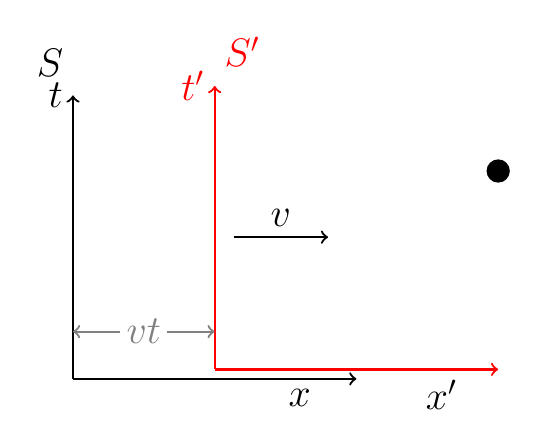
\begin{tikzpicture}[
    scale=1.2,          % Escala general de la figura
    font=\Large,        % Tamaño de la fuente para las etiquetas
    axis/.style={->, thick}, % Estilo para los ejes (flecha, grueso)
]

% --- Sistema de referencia S (estacionario, en gris) ---
% Eje horizontal x
\draw[axis, black] (0,0) -- (3,0) node[below, black, pos=0.8] {$x$};
% Eje vertical t
\draw[axis, black] (0,0) -- (0,3) node[left] {$t$};
% Etiqueta del sistema
\node[black, anchor=south east] at (0,3.1) {$S$};

% --- Sistema de referencia S' (en movimiento, en rojo) ---
% Usamos un 'scope' con 'xshift' para mover todo el sistema S'
\begin{scope}[xshift=1.5cm,yshift=0.1cm]
    % Eje horizontal x'
    \draw[axis, red] (0,0) -- (3,0) node[below, black, pos=0.8] {$x'$};
    % Eje vertical t'
    \draw[axis, red] (0,0) -- (0,3) node[left] {$t'$};
    % Etiqueta del sistema
    \node[red, anchor=south west] at (0,3.1) {$S'$};
\end{scope}

% --- Flecha de velocidad v ---
\draw[axis, black] (1.7, 1.5) -- (2.7, 1.5) node[midway, above] {$v$};

% --- Punto del evento ---
\fill[black] (4.5, 2.2) circle (3.5pt);

% --- distancia entre sistemas ---
\draw[axis, gray] (0.5, 0.5) -- (0.0, 0.5) node[midway, ,gray,pos=-0.5] {$vt$};
\draw[axis, gray] (1.0, 0.5) -- (1.5, 0.5);



\end{tikzpicture}
%\end{center}
% --- Fin del código TikZ ---
    \caption{Sistema de referencia inercial $\color{red}S'$, a velocidad constante en $x$, $v$, con respecto al sistema en reposo $S$. A un tiempo $t$ el origin de $\color{red}S'$ se encuentra a una distancia $x = vt$ del origen de $S$. }
    \label{fig:placeholder}
\end{figure}


Ahora nos enfocamos en derivar las transformaciones para $x'$ y $t'$.

\section{Pasos de la Derivación}

\subsection{Paso 1: La Suposición de Linealidad}

Las transformaciones deben ser lineales para preservar el principio de inercia. Un movimiento uniforme en un sistema debe aparecer como un movimiento uniforme en el otro. Por lo tanto, las transformaciones tienen la forma:
\begin{align}
\label{eq:tl1}
 x' = Ax + Bt\,.   
\end{align}
 
\subsection{Paso 2: Usando el Movimiento del Origen}

El origen de $S'$ ($x'=0$) se mueve con velocidad $v$ en el sistema $S$, por lo que su posición es $x=vt$. Sustituyendo esto en la ecuación~\eqref{eq:tl1}:
\[ 0 = A(vt) + Bt \implies B = -Av \]
Esto da $x' = A(x-vt)$. Renombramos la constante $A$ con el símbolo más convencional $\gamma$.
\begin{align}
\label{eq:xplt}
x' = \gamma (x - vt).    
\end{align}

\subsection{Paso 3: Aplicando el Principio de Relatividad}

La transformación inversa (de $S'$ a $S$) debe tener la misma forma, con la velocidad invertida ($v \to -v$):
\begin{align}
\label{eq:invxplt}
    x = \gamma (x' + vt').
\end{align}

\subsection{Paso 4: Aplicando el Segundo Postulado}
Imaginemos un pulso de luz emitido desde el origen en $t=t'=0$. Un observador en $S$ ve su frente de onda en $x=ct$, mientras que un observador en $S'$ lo ve en $x'=ct'$. Sustituyendo esto en nuestras ecuaciones de transformación:

\newcounter{paso}

\noindent
%\renewcommand{\arraystretch}{1.5}
\begin{tabular}{l|p{0.35\textwidth}|p{0.6\textwidth}}
\textbf{Paso}&\textbf{Encontrar} $\gamma$& \textbf{Paso algebraico} \\\hline
\stepcounter{paso}\thepaso)&$\begin{aligned}
    x' =& \gamma (x - vt),\\
    x = &\gamma (x' + vt').
\end{aligned}$& Ecuaciones \eqref{eq:xplt} y \eqref{eq:invxplt}\\\hline
\stepcounter{paso}\thepaso)&$\begin{aligned}[t]
ct' &= \gamma(ct - vt) = \gamma t (c-v)   \\
ct &= \gamma(ct' + vt') = \gamma t' (c+v)  
\end{aligned}$  &  Reemplazando $x=ct$ y $x'=ct'$ en  
las ecuaciones anteriores\\\hline
\stepcounter{paso}\thepaso)&$(ct')(ct) = [\gamma t (c-v)][\gamma t' (c+v)]$& Multiplicando las dos ecuaciones\\\hline
\stepcounter{paso}\thepaso)&$c^2 t' t = \gamma^2 t t' (c-v)(c+v)$& 
Realizando las operaciones indicadas\\\hline
\stepcounter{paso}\thepaso)&$c^2= \gamma^2 (c^2-v^2)$& Dividiendo por $tt'$ a ambos lados de la igualdad y expandiendo la diferencia de cuadrados \\\hline
\stepcounter{paso}\thepaso)&$1=\gamma^2(1-v^2/c^2)$&Dividiendo por $c^2$ a ambos lados de la igualdad.\\\hline
\stepcounter{paso}\thepaso)&$\gamma^2 = \dfrac{1}{1-v^2/c^2}$&
Dividiendo por $1-v^2/c^2$ a ambos lados de la igualdad.
\\[8pt]\hline
\stepcounter{paso}\thepaso)&$\gamma = \dfrac{1}{\sqrt{1-v^2/c^2}}$&
Sacando raíz cuadrada a ambos lados iguales\\[8pt]\hline
\end{tabular}

De ésta forma:
\begin{align}
\label{eq:gamma}
    \boxed{\gamma = \frac{1}{\sqrt{1 - v^2/c^2}}} \,,
\end{align}
y 
\begin{align}
\label{eq:gammasquare}
    \gamma^2 =&\frac{1}{1-\dfrac{v^2}{c^2}} =  \frac{c^2}{c^2-v^2}\,.
\end{align}

\subsection{Paso 6: Derivando la Transformación del Tiempo}
Dado que ya tenemos la expresión completa para $x'$, en las ecuaciones \eqref{eq:xplt} y \eqref{eq:invxplt}, podemos
despejar $t'$

\noindent
\setcounter{paso}{0}
\begin{tabular}{l|p{0.35\textwidth}|p{0.6\textwidth}}
\textbf{paso} &\textbf{Despejar} $t'$& \textbf{Paso algebraico} \\\hline
\stepcounter{paso}\thepaso) & $\begin{aligned}
    x' =& \gamma (x - vt),\\
    x = &\gamma (x' + vt').
\end{aligned}$& Ecuaciones \eqref{eq:xplt} y \eqref{eq:invxplt}\\\hline
\stepcounter{paso}\thepaso) & $x=\gamma[\gamma(x-vt) +v t']$&sustituyendo $x'=\gamma(x-vt)$ en $x = \gamma(x' + vt')$\\\hline
\stepcounter{paso}\thepaso) & $x=\gamma^2x-\gamma^2 vt +\gamma v t'$  & Expandiendo el lado derecho\\\hline
\stepcounter{paso}\thepaso) & $\gamma v t' = x-\gamma^2x +\gamma^2 v t$ & Sumando $-\gamma^2x +\gamma^2 v t$ a ambos lados de la igualdad. \\\hline
\stepcounter{paso}\thepaso) & $\gamma v t' = x(1-\gamma^2) +\gamma^2 v t$  & Factorizando $x$.\\\hline
\stepcounter{paso}\thepaso) & $\gamma v t' = x\left(1-\dfrac{c^2}{c^2-v^2}\right) +\gamma^2 v t$ & Reemplazando $\gamma^2$ de la ecuación~\eqref{eq:gammasquare} \\\hline
\stepcounter{paso}\thepaso) & $\gamma v t' = x\left(\dfrac{\cancel{c^2}-v^2-\cancel{c^2}}{c^2-v^2}\right) +\gamma^2 v t$. & Sumando las fracciones.\\\hline
\stepcounter{paso}\thepaso) & $\gamma v t' =\gamma^2 v t- xv^2\left[\dfrac{c^2}{c^2(c^2-v^2)}\right]$ & Multiplicando y dividiendo por $c^2$ en el último término. \\[5pt]\hline
\stepcounter{paso}\thepaso) & $\cancel{\gamma}\cancel{v}  t' =\gamma^{\cancel{2}}\cancel{v}  t- \gamma^{\cancel{2}} \dfrac{v^{\cancel{2}} x}{c^2}$  &
Usando de nuevo la ecuación~\eqref{eq:gammasquare} para $\gamma^2$ y cancelando términos iguales a ambos lados de la igualdad\\\hline
\stepcounter{paso}\thepaso) & $t' = \gamma\left(t-\dfrac{vx}{c^2}\right)$\\[5pt]\hline
\end{tabular}

De modo que
\[ \boxed{t' = \gamma \left( t - \frac{vx}{c^2} \right)} \]

\section{Resumen de las Transformaciones de Lorentz}
Las transformaciones de Lorentz completas son:
\[
\boxed{
\begin{aligned}
t' &= \gamma \left( t - \frac{vx}{c^2} \right) \\
x' &= \gamma (x - vt) \\
y' &= y \\
z' &= z
\end{aligned}
}
\]

\section{Las Transformaciones Inversas}
Las transformaciones de $S'$ a $S$ se encuentran intercambiando las coordenadas y haciendo $v \to -v$:
\[
\boxed{
\begin{aligned}
t &= \gamma \left( t' + \frac{vx'}{c^2} \right) \\
x &= \gamma (x' + vt') \\
y &= y' \\
z &= z'
\end{aligned}
}
\]

\subsection{Transformaciones de Galileo}
Se obtienen cuando no hay una velocidad límite, y por lo tanto $c\to \infty$
\begin{align*}
t' &= \lim_{c\to\infty}\left[\gamma \left( t - \frac{vx}{c^2} \right)\right] 
    = t\\
x' &= \lim_{c\to\infty}\left[\gamma (x - vt)\right]  = x - vt \\
y' &= y \\
z' &= z
\end{align*}

Mientras que para factor de Lorentz $\gamma$, o el factor de contracción relativista $1/\gamma$, 
\begin{align}
    \lim_{c\to\infty}\ \gamma = 1\,. 
\end{align}

Esto quiere decir que las las distancia y tiempos no están afectados por las transformaciones de Galileo.




% --- INFORMACIÓN DEL TÍTULO ---
\section{Derivación de las Transformaciones de Lorentz a partir de Simetrías del Espacio--tiempo}
\subsection{El Enfoque de Ignatowski}
Este documento presenta una derivación de las transformaciones de Lorentz basada en principios fundamentales de simetría, en lugar de postular la constancia de la velocidad de la luz. Este enfoque, a veces llamado la derivación de Ignatowski, se basa en el Principio de Relatividad y la homogeneidad e isotropía del espaciotiempo. Mostraremos que estos principios conducen lógicamente a la existencia de una velocidad universal e invariante, que identificamos con la velocidad de la luz.

Ver \cite{Datta:2022cpw} %https://inspirehep.net/literature/2611550


\subsection{Principios Fundamentales}
La derivación se basa en tres supuestos centrales:
\begin{enumerate}
    \item \textbf{El Principio de Relatividad:} Las leyes de la física son las mismas en todos los sistemas de referencia inerciales.
    \item \textbf{Homogeneidad del Espaciotiempo:} Las leyes de la física son independientes de la posición en el espacio y el tiempo.
    \item \textbf{Isotropía del Espacio:} Las leyes de la física son independientes de la dirección.
\end{enumerate}


\subsection{Paso 1: Linealidad a partir de la Homogeneidad}
Consideremos dos sistemas de referencia inerciales, $S(x,t)$ y $S'(x',t')$, con $S'$ moviéndose a una velocidad $v$ relativa a $S$ a lo largo del eje x. Buscamos las funciones de transformación $x' = f(x,t)$ y $t' = g(x,t)$.

La homogeneidad del espaciotiempo implica que las ecuaciones de transformación deben ser \textbf{lineales}. Si no lo fueran, un movimiento uniforme en un sistema (una línea recta en un diagrama de espaciotiempo) aparecería como un movimiento acelerado en otro. Esto significaría que las leyes de la física dependerían de la elección del origen, violando la homogeneidad. Por lo tanto, la forma más general de las transformaciones debe ser lineal:
\begin{align*}
x' &= Ax + Bt \\
t' &= Dx + Et
\end{align*}
donde los coeficientes $A, B, D, E$ solo pueden depender de la velocidad relativa, $v$.

\subsection{Paso 2: Usando Cinemática Básica}
Podemos simplificar los coeficientes usando el movimiento de los orígenes de los sistemas.
\begin{itemize}
    \item El origen del sistema $S'$ ($x'=0$) se mueve con velocidad $v$ en el sistema $S$. Su posición en $S$ es por lo tanto $x=vt$. Sustituyamos esto en nuestra primera ecuación:
    \[ 0 = A(vt) + Bt \implies 0 = (Av+B)t \]
    Esto debe ser válido para todo tiempo $t$, por lo que debemos tener $B = -Av$. La transformación para $x'$ se convierte en:
    \[ x' = Ax - Avt = A(x-vt) \]
\end{itemize}
Renombremos el coeficiente $A(v)$ con la notación más familiar $\gamma(v)$.
\begin{equation} \label{eq:x_prime}
x' = \gamma(v)(x - vt)
\end{equation}

\subsection{Paso 3: Aplicando la Relatividad y la Isotropía}
El Principio de Relatividad establece que la transformación de $S'$ de vuelta a $S$ debe tener exactamente la misma forma matemática. La única diferencia es que desde la perspectiva de $S'$, el sistema $S$ se mueve con velocidad $-v$. Por lo tanto, la transformación inversa debe ser:
\begin{equation} \label{eq:x}
x = \gamma(-v)(x' + vt')
\end{equation}
Ahora, invocamos la \textbf{isotropía del espacio}. La isotropía significa que la física no debe depender de la dirección del vector velocidad. Por lo tanto, cualquier efecto físico de la transformación solo puede depender de la \textit{rapidez}, $|v|$, no de la dirección de la velocidad. Esto implica:
\[ \gamma(v) = \gamma(-v) \]
Esto simplifica nuestro par de transformaciones a:
\begin{align*}
x' &= \gamma(v)(x - vt) \\
x &= \gamma(v)(x' + vt')
\end{align*}

\subsection{Paso 4: Encontrando la Transformación del Tiempo}
Todavía necesitamos determinar la transformación para el tiempo. Podemos mostrar que debe tomar la forma simétrica:
\begin{equation} \label{eq:t_prime}
t' = \gamma(v)(t - \alpha(v) x)
\end{equation}
donde $\alpha(v)$ es alguna función de la velocidad. Por el Principio de Relatividad, la transformación inversa debe ser:
\begin{equation} \label{eq:t}
t = \gamma(v)(t' + \alpha(v) x')
\end{equation}
Nótese que la isotropía implica $\alpha(-v) = -\alpha(v)$ (debe ser una función impar).

\subsection{Paso 5: La Propiedad de Grupo y la Constante Universal}
Este es el paso crucial que reemplaza el postulado de la velocidad de la luz. Consideremos tres sistemas: $S$, $S'$ y $S''$. Sea la velocidad de $S'$ relativa a $S$ $v_1$, y la velocidad de $S''$ relativa a $S'$ $v_2$. La composición de estas dos transformaciones debe dar como resultado una transformación de la misma forma.

Sustituyendo (\ref{eq:x_prime}) y (\ref{eq:t_prime}) en (\ref{eq:x}) y (\ref{eq:t}), podemos resolver para las funciones. Un método más directo es requerir consistencia entre las transformaciones. Sustituyamos (\ref{eq:x_prime}) en (\ref{eq:x}):
\begin{align*}
x &= \gamma(v)(x' + vt') \\
x &= \gamma(v)[\gamma(v)(x-vt) + v t']
\end{align*}
Ahora sustituimos nuestra expresión para $t'$ (\ref{eq:t_prime}):
\begin{align*}
x &= \gamma(v)[\gamma(v)(x-vt) + v \gamma(v)(t - \alpha(v)x)] \\
x &= \gamma(v)^2 [ (x-vt) + v(t-\alpha(v)x) ] \\
x &= \gamma(v)^2 [ x - vt + vt - v\alpha(v)x ] \\
x &= \gamma(v)^2 x (1 - v\alpha(v))
\end{align*}
Como esto debe ser válido para cualquier $x$, debemos tener:
\[ 1 = \gamma(v)^2 (1 - v\alpha(v)) \]
Esto relaciona nuestras dos funciones desconocidas, $\gamma(v)$ y $\alpha(v)$.

A partir del argumento de la propiedad de grupo (considerando tres sistemas), se puede mostrar que la razón $\alpha(v)/v$ debe ser una constante universal, independiente del sistema de referencia. Llamemos a esta constante $K$.
\[ \frac{\alpha(v)}{v} = K \implies \alpha(v) = Kv \]
Ahora sustituimos esto de nuevo en nuestra relación de consistencia:
\[ 1 = \gamma(v)^2 (1 - v(Kv)) = \gamma(v)^2 (1 - K v^2) \]
Resolviendo para $\gamma(v)$:
\[ \boxed{\gamma(v) = \frac{1}{\sqrt{1 - K v^2}}} \]

\subsection{Paso 6: La Naturaleza Física de la Constante \texorpdfstring{$K$}{K}}
Hemos derivado la forma completa de las transformaciones basándonos únicamente en principios de simetría. La física está contenida en la constante universal $K$.
\begin{enumerate}
    \item \textbf{Caso 1: $K=0$} \\
    Si $K=0$, entonces $\gamma = 1$ y $\alpha=0$. Las transformaciones se convierten en $x' = x - vt$ y $t'=t$. Esta es la \textbf{transformación de Galileo}. En este universo, no hay límite de velocidad.

    \item \textbf{Caso 2: $K<0$} \\
    Si $K$ es negativo, sea $K = -1/R^2$. Entonces $\gamma = 1/\sqrt{1+v^2/R^2}$. Esto corresponde a transformaciones en un espacio euclidiano 4D (rotaciones). Esto es matemáticamente posible pero no describe nuestro universo.

    \item \textbf{Caso 3: $K>0$} \\
    Si $K$ es positivo, debe tener unidades de (1/velocidad$^2$). Definamos una nueva constante $c$ tal que $K = 1/c^2$. Esta constante $c$ debe ser una velocidad universal e invariante. El factor de Lorentz y las transformaciones se convierten en:
    \[ \gamma = \frac{1}{\sqrt{1 - v^2/c^2}} \]
    \[ x' = \gamma(x-vt) \]
    \[ t' = \gamma(t - \frac{v}{c^2}x) \]
    Estas son las \textbf{transformaciones de Lorentz}.
\end{enumerate}

\subsection{Conclusión}
Sin asumir nunca que la luz viaja a una velocidad constante, hemos demostrado que las simetrías fundamentales del espaciotiempo (homogeneidad e isotropía) y el principio de relatividad conducen a una conclusión sorprendente: \textbf{debe existir una velocidad universal e invariante en nuestro universo}.

Toda la evidencia experimental, desde el electromagnetismo hasta la desintegración de partículas, confirma que vivimos en un universo donde $K > 0$. Llamamos a esta velocidad universal $c$, y la identificamos con la velocidad de la luz en el vacío. La constancia de la velocidad de la luz no es una suposición separada, sino una consecuencia directa de la estructura del espaciotiempo mismo.

\section{Derivación de la Dilatación del Tiempo a partir de las Transformaciones de Lorentz}

En las aplicaciones prácticas, donde se estudia el movimiento de un cuerpo a velocidad constante, es conveniente asumir que el sistema inercial se mueve con la misma velocidad del cuerpo bajo estudio, como se ilustra en la figura~\ref{fig:movv}.

\begin{figure}
% --- Inicio del código TikZ para insertar ---
%\begin{center}
\centering
\begin{tikzpicture}[
    scale=1.2,          % Escala general de la figura
    font=\Large,        % Tamaño de la fuente para las etiquetas
    axis/.style={->, thick}, % Estilo para los ejes (flecha, grueso)
]

% --- Sistema de referencia S (estacionario, en gris) ---
% Eje horizontal x
\draw[axis, black] (0,0) -- (3,0) node[below, black, pos=0.8] {$x$};
% Eje vertical t
\draw[axis, black] (0,0) -- (0,3) node[left] {$t$};
% Etiqueta del sistema
\node[black, anchor=south east] at (0,3.1) {$S$};

% --- Sistema de referencia S' (en movimiento, en rojo) ---
% Usamos un 'scope' con 'xshift' para mover todo el sistema S'
\begin{scope}[xshift=1.5cm,yshift=0.1cm]
    % Eje horizontal x'
    \draw[axis, red] (0,0) -- (3.5,0) node[below, black, pos=0.8] {$x'$};
    % Eje vertical t'
    \draw[axis, red] (0,0) -- (0,3) node[left] {$t'$};
    % Etiqueta del sistema
    \node[red, anchor=south west] at (0,3.1) {$S'$};
\end{scope}

% --- Flecha de velocidad v ---
\draw[axis, black] (1.7, 1.5) -- (2.7, 1.5) node[midway, above] {$v$};

% --- Punto del evento ---
\fill[black] (1.7, 1.5) circle (3.5pt);

\node[inner sep=0pt] (russell) at (3.5,2)
    {\includegraphics[scale=0.03]{clock}};

\draw[dotted] (3.5, 0.1) -- (3.5,2);

\node[black] (russell) at (3.5,-0.15) {$x'_c$};

\draw[axis, black] (3.7, 2) -- (4.7, 2) node[midway, above] {$v$};


\end{tikzpicture}
%\end{center}
% --- Fin del código TikZ ---
    \caption{Sistema de referencia inercial $\color{red}S'$, moviendos con velocidad constante en $x$, $v$, con el objeto bajo estudio }
    \label{fig:movv}
\end{figure}


La dilatación del tiempo es una consecuencia directa y famosa de las transformaciones de Lorentz. Describe el fenómeno en el que un reloj que está en movimiento relativo a un observador se mide por ese observador como si estuviera marcando el tiempo más lentamente que un reloj que está en reposo relativo a él.

Para derivar esto, estableceremos un experimento mental simple y aplicaremos la transformación de Lorentz para el tiempo.

\subsection{La Configuración Física (Experimento Mental)}

\begin{enumerate}
    \item \textbf{Dos Sistemas:} Tenemos dos sistemas inerciales, $S$ y $S'$. Como antes, el sistema $S$ es el sistema ``estacionario" (por ejemplo, un observador en el suelo), y el sistema $S'$ se mueve con una velocidad constante $v$ a lo largo del eje x relativo a $S$.

    \item \textbf{Un Reloj en el Sistema en Movimiento:} Imaginemos que hay un reloj en reposo en el sistema en movimiento, $S'$. Dado que el reloj no se mueve \textit{dentro de su propio sistema}, su posición es un valor constante, que llamaremos $x'_c$.

    \item \textbf{Dos Eventos:} Consideraremos dos eventos, que son dos "tictacs" consecutivos de este reloj.
    \begin{itemize}
        \item \textbf{Evento 1:} El reloj hace tictac por primera vez. Desde la perspectiva de un observador en el sistema $S'$, este evento ocurre en las coordenadas $(t'_1, x'_c)$.
        \item \textbf{Evento 2:} El reloj hace tictac por segunda vez. En el sistema $S'$, este evento ocurre en las coordenadas $(t'_2, x'_c)$.
    \end{itemize}
\end{enumerate}

\subsection{Definiendo el Tiempo Propio}

El intervalo de tiempo entre dos eventos que ocurren en la \textbf{misma ubicación espacial} en un sistema dado se llama \textbf{intervalo de tiempo propio}, denotado por $\Delta t_0$.

En nuestra configuración, los dos tictacs del reloj ocurren en la misma ubicación ($x'_c$) en el sistema $S'$. Por lo tanto, el intervalo de tiempo medido por un observador en el sistema en movimiento $S'$ es el tiempo propio:
\[ \Delta t_0 = t'_2 - t'_1 \]
Nuestro objetivo es encontrar el intervalo de tiempo entre estos mismos dos eventos según lo medido por el observador en el sistema estacionario $S$. Llamemos a este intervalo $\Delta t$.
\[ \Delta t = t_2 - t_1 \]

\subsection{Aplicando las Transformaciones de Lorentz}

Necesitamos relacionar las coordenadas de tiempo en $S$ con las coordenadas en $S'$. La transformación de Lorentz inversa para el tiempo es la opción más conveniente aquí, ya que expresa el tiempo del sistema estacionario ($t$) en términos de las coordenadas del sistema en movimiento ($t', x'$).
\[ t = \gamma \left( t' + \frac{vx'}{c^2} \right) \]
Ahora, aplicamos esta transformación a nuestros dos eventos:
\begin{enumerate}
    \item El tiempo del Evento 1 medido en el sistema $S$ es $t_1$:
    \[ t_1 = \gamma \left( t'_1 + \frac{vx'_c}{c^2} \right) \]
    \item El tiempo del Evento 2 medido en el sistema $S$ es $t_2$:
    \[ t_2 = \gamma \left( t'_2 + \frac{vx'_c}{c^2} \right) \]
\end{enumerate}

\subsection{La Derivación}

El intervalo de tiempo $\Delta t$ medido por el observador en el sistema $S$ es la diferencia entre $t_2$ y $t_1$.
\begin{align*}
\Delta t &= t_2 - t_1 \\
&= \left[ \gamma \left( t'_2 + \frac{vx'_c}{c^2} \right) \right] - \left[ \gamma \left( t'_1 + \frac{vx'_c}{c^2} \right) \right] \\
&= \gamma \left( t'_2 + \frac{vx'_c}{c^2} - t'_1 - \frac{vx'_c}{c^2} \right) \\
&= \gamma (t'_2 - t'_1)
\end{align*}
El término que involucra la posición $x'_c$ se cancela precisamente porque el reloj estaba en reposo en el sistema $S'$. Ahora sustituimos la definición de tiempo propio, $\Delta t_0 = t'_2 - t'_1$:
\[ \Delta t = \gamma \Delta t_0 \]

\subsection{Resultado e Interpretación}

La fórmula final para la dilatación del tiempo se obtiene sustituyendo la expresión para $\gamma$:
\[ \boxed{ \Delta t = \frac{\Delta t_0}{\sqrt{1 - v^2/c^2}} } \]
Interpretemos este importante resultado:
\begin{itemize}
    \item El factor de Lorentz $\gamma = \frac{1}{\sqrt{1 - v^2/c^2}}$ es siempre mayor o igual a 1, ya que la velocidad $v$ debe ser menor que $c$.
    \item Esto significa que $\Delta t \ge \Delta t_0$.
    \item El intervalo de tiempo ($\Delta t$) medido por el observador en el sistema ``estacionario" $S$ es \textit{más largo} que el intervalo de tiempo propio ($\Delta t_0$) medido en el sistema de reposo del reloj.
\end{itemize}
Un intervalo de tiempo más largo entre tictacs significa que se observa que el reloj funciona más lentamente. Por lo tanto, el observador en $S$ concluye que el reloj en movimiento funciona lentamente en comparación con su propio reloj idéntico. Este fenómeno es la \textbf{dilatación del tiempo}.


\section{Derivación de la Contracción de la Longitud a partir de las Transformaciones de Lorentz}

\begin{figure}
% --- Inicio del código TikZ para insertar ---
%\begin{center}
\centering
\begin{tikzpicture}[
    scale=1.2,          % Escala general de la figura
    font=\Large,        % Tamaño de la fuente para las etiquetas
    axis/.style={->, thick}, % Estilo para los ejes (flecha, grueso)
]

% --- Sistema de referencia S (estacionario, en gris) ---
% Eje horizontal x
\draw[axis, black] (0,0) -- (4,0) node[below, black, pos=0.5] {$x$};
% Eje vertical t
\draw[axis, black] (0,0) -- (0,3) node[left] {$t$};
% Etiqueta del sistema
\node[black, anchor=south east] at (0,3.1) {$S$};

% --- Sistema de referencia S' (en movimiento, en rojo) ---
% Usamos un 'scope' con 'xshift' para mover todo el sistema S'
\begin{scope}[xshift=1.5cm,yshift=0.1cm]
    % Eje horizontal x'
    \draw[axis, red] (0,0) -- (3.5,0) node[below, black, pos=0.8] {$x'$};
    % Eje vertical t'
    \draw[axis, red] (0,0) -- (0,3) node[left] {$t'$};
    % Etiqueta del sistema
    \node[red, anchor=south west] at (0,3.1) {$S'$};
\end{scope}

% --- Flecha de velocidad v ---
\draw[axis, black] (1.7, 1.5) -- (2.7, 1.5) node[midway, above] {$v$};

% --- Punto del evento ---
\fill[black] (1.7, 1.5) circle (3.5pt);

\node[inner sep=0pt] (russell) at (3.32,2)
    {\includegraphics[scale=0.1]{ruler}};


\draw[dotted] (2.95, -0.2) -- (2.95,2);
\node[black] (russell) at (2.95,-0.2) {$x_1$};

\draw[dotted] (3.7, -0.2) -- (3.7,2);
\node[black] (russell) at (3.7,-0.2) {$x_2$};


\draw[axis, black] (3.7, 2) -- (4.7, 2) node[midway, above] {$v$};

% --- distancia entre sistemas ---
\draw[axis, gray] (3.15, 0.5) -- (2.95, 0.5) node[midway, ,gray,pos=-0.8] {$t$};
\draw[axis, gray] (3.5, 0.5) -- (3.7, 0.5);



\end{tikzpicture}
%\end{center}
% --- Fin del código TikZ ---
    \caption{Sistema de referencia inercial $\color{red}S'$, moviendos con velocidad constante en $x$, $v$, con el objeto bajo estudio }
    \label{fig:movruler}
\end{figure}




La contracción de la longitud es otra predicción fundamental de la Relatividad Especial. Afirma que se mide que un objeto en movimiento es más corto a lo largo de su dirección de movimiento que su longitud cuando se mide en reposo. Este efecto también se conoce como contracción de Lorentz.

La clave para medir correctamente la longitud de un objeto en movimiento es determinar las posiciones de sus dos extremos \textbf{simultáneamente} en el sistema de referencia del observador.

\subsection{La Configuración Física (Experimento Mental)}

\begin{enumerate}
    \item \textbf{Dos Sistemas:} Como siempre, consideramos un sistema estacionario $S$ (el sistema del observador) y un sistema $S'$ que se mueve con una velocidad constante $v$ a lo largo del eje x positivo relativo a $S$.

    \item \textbf{Un Objeto en el Sistema en Movimiento:} Colocamos un objeto, como una varilla, en reposo en el sistema en movimiento $S'$. La varilla está alineada a lo largo del eje x'.
    \begin{itemize}
        \item La posición del primer extremo de la varilla en el sistema $S'$ es $x'_1$.
        \item La posición del segundo extremo de la varilla en el sistema $S'$ es $x'_2$.
    \end{itemize}
\end{enumerate}

\subsection{Definiendo la Longitud Propia}

La longitud de un objeto medida en el sistema de referencia donde está en reposo se llama su \textbf{longitud propia}, denotada por $L_0$.

En nuestra configuración, la varilla está en reposo en el sistema $S'$. Por lo tanto, su longitud propia es la simple diferencia entre las coordenadas de sus extremos en ese sistema:
\[ L_0 = x'_2 - x'_1 \]
Nuestro objetivo es encontrar la longitud de esta misma varilla según lo medido por un observador en el sistema estacionario $S$. Llamemos a esta longitud medida $L$.

\subsection{Midiendo la Longitud en el Sistema Estacionario}

Para medir la longitud $L$ de la varilla en movimiento, el observador en el sistema $S$ debe localizar las posiciones de sus dos extremos, $x_1$ y $x_2$, en el mismo instante de tiempo, $t$.
\begin{itemize}
    \item La medición de la posición del primer extremo, $x_1$, ocurre en el tiempo $t$.
    \item La medición de la posición del segundo extremo, $x_2$, ocurre en el mismo tiempo $t$.
\end{itemize}
La longitud medida por el observador en el sistema $S$ es por lo tanto:
\[ L = x_2 - x_1 \]

\subsection{Aplicando las Transformaciones de Lorentz}

Necesitamos una transformación de Lorentz que conecte las coordenadas en $S$ y $S'$. La transformación para la coordenada espacial $x'$ es la más directa de usar:
\[ x' = \gamma (x - vt) \]
Aplicamos esta transformación a los dos extremos de la varilla.
\begin{enumerate}
    \item Para el primer extremo de la varilla (coordenadas $x'_1$ y $x_1$):
    \[ x'_1 = \gamma (x_1 - vt) \]
    \item Para el segundo extremo de la varilla (coordenadas $x'_2$ y $x_2$):
    \[ x'_2 = \gamma (x_2 - vt) \]
\end{enumerate}
Nótese que el tiempo $t$ es el mismo en ambas ecuaciones porque las mediciones se realizan simultáneamente en el sistema $S$.

\subsection{La Derivación}

Ahora, podemos encontrar la longitud propia $L_0$ restando la primera ecuación de la segunda:
\begin{align*}
x'_2 - x'_1 &= \left[ \gamma (x_2 - vt) \right] - \left[ \gamma (x_1 - vt) \right] \\
&= \gamma (x_2 - vt - x_1 + vt) \\
&= \gamma (x_2 - x_1)
\end{align*}
El término $vt$ se cancela, lo que confirma que nuestra elección del tiempo específico de medición no afecta el resultado.

Ahora, sustituimos las definiciones de longitud propia ($L_0 = x'_2 - x'_1$) y longitud medida ($L = x_2 - x_1$):
\[ L_0 = \gamma L \]
Para encontrar la longitud medida $L$, reorganizamos la ecuación:
\[ L = \frac{L_0}{\gamma} \]

\subsection{Resultado e Interpretación}

Sustituyendo la expresión completa para el factor de Lorentz $\gamma = \frac{1}{\sqrt{1-v^2/c^2}}$ se obtiene la fórmula final para la contracción de la longitud:
\[ \boxed{ L = L_0 \sqrt{1 - v^2/c^2} } \]
Interpretemos este resultado:
\begin{itemize}
    \item El factor $\sqrt{1 - v^2/c^2}$ es siempre menor o igual a 1.
    \item Esto significa que $L \le L_0$.
    \item La longitud ($L$) de la varilla medida por el observador en el sistema $S$ es \textit{más corta} que su longitud propia ($L_0$) medida en su sistema de reposo.
\end{itemize}
Es crucial notar que esta contracción \textbf{solo ocurre a lo largo de la dirección del movimiento}. Las longitudes en las direcciones perpendiculares al movimiento (y y z) no se ven afectadas, porque las transformaciones de Lorentz para esas coordenadas son simplemente $y' = y$ y $z' = z$.

ver \url{https://inspirehep.net/literature/2825885}

\section{Forma Vectorial y Rapidez}

%\subsection{Unidades Naturales y Rapidez}
Para tener las coordenadas con las mismas unidades,, debemos usar $ct$ paraque seae sea interpretado como una dimensión espacial
\begin{align}
ct' =& \gamma\left(ct-\frac{v}{c}x\right),\\
x'=&\gamma\left(x-\frac{v}{c}ct\right)
\end{align}


\subsection{Funciones Hiperbólicas}
\begin{align*}
    \cosh x =& \frac{{e}^{x}+{e}^{-x}}{2}\,,&
\sinh x =& \frac{{e}^{x}-{e}^{-x}}{2}\,.
\end{align*}
Por lo tanto
\begin{align*}
    \cosh^2x - \sinh^2x =& \frac{({e}^{x}+{e}^{-x})^2
    -({e}^{x}-{e}^{-x})^2}{4}\\
    =&\frac{{e}^{2x}+2{e}^{x}{e}^{-x}+{e}^{-2x}
-({e}^{2x}-2{e}^{x}{e}^{-x}+{e}^{-2x})}{4}\\
=&\frac{\cancel{{e}^{2x}}+2+\cancel{{e}^{-2x}}
-\cancel{{e}^{2x}}+2-\cancel{{e}^{-2x}}}{4}\\
=&\frac{4}{4}\\
=&1
\end{align*}

Podemos parametrizar la velocidad usando la \textbf{rapidez}, $\xi$:
\[ \gamma = \cosh\xi, \quad \frac{v}{c}\gamma = \sinh\xi \]
Esta parametrización es válida porque satisface automáticamente la identidad $\gamma^2(1-v^2)=1$:
\[ \cosh^2\xi - \sinh^2\xi = \gamma^2 - \left(\frac{v}{c}\gamma\right)^2 = \gamma^2\left(1-\frac{v^2}{c^2}\right) = 1 \]
A partir de esto, también encontramos que la velocidad está relacionada con la rapidez por 
\begin{align*}
    \frac{v}{c} = \tanh\xi\,,
\end{align*}
donde
\begin{align*}
\tanh\xi \equiv \frac{\sinh\xi}{\cosh\xi}\,.    
\end{align*}

En resumen, las transformaciones de Lorentz se pueden escribir como
\[
\boxed{
\begin{aligned}    
    ct' =& ct\cosh\xi - x\sinh\xi \\
    x' = &x\cosh\xi -ct\sinh\xi\\
    y' = & y\\
    z' = &z\,.
\end{aligned}
}
\]

Si definimos la coordenada temporal en la dimensiones de distancia como $x^0\equiv ct$, podemos definir el cuadrivector
\begin{align}
    x^\mu \equiv \left(x^0, x^1, x^2,x^3 \right) = \left(ct, x, y,z \right)
\end{align}
y
\[
\boxed{
\begin{aligned}    
    {x^0}' =& x^0\cosh\xi - x^1\sinh\xi \\
    {x^1}' = &x^1\cosh\xi -x^0\sinh\xi\\
    {x^2}' = & x^2\\
    {x^3}' = &x^3\,.
\end{aligned}
}
\]

A continuación trabajaremos en dos dimensiones, una temporal y una espacial, a saber
\begin{align}
    x^\mu \equiv \left(x^0, x^1 \right) = \left(ct, x \right)
\end{align}

\section{Invariancia}
Para rotaciones tenemos el vector de posición de la figura~\ref{fig:rot}
\begin{align*}
    \boldsymbol{r}' = (x',y')=  (x\cos\theta+y\sin\theta,y\cos\theta-x\sin\theta).
\end{align*}

\begin{figure}
    \centering
    \includegraphics[width=1\linewidth]{so2}
    \caption{Rotación de coordenadas}
    \label{fig:rot}
\end{figure}

El módulo de este vector es invariante

\begin{align*}
    \boldsymbol{r}'\cdot\boldsymbol{r}' =&{x'}^2+{y'}^2  \\
    =&(x\cos\theta+y\sin\theta)^2+(y\cos\theta-x\sin\theta)^2\\
    = & x^2+y^2\,.
\end{align*}
Verifiquemos, bajo qué condiciones el módulo del vector de impulso es invariante bajo transformaciones de Lorentz. Definimos el producto escalar entre dos vectores
$\boldsymbol{b} = (b_1,b_2)$ y $\boldsymbol{c} = (c_1,c_2) $ como
\begin{align}
    \boldsymbol{b} \cdot \boldsymbol{c} = g_{1} b_1 c_1 + g_{2} b_2 c_2\,.
\end{align}
con $g_{1}$ y $g_{2}$ a ser fijados. 

Con esta definición el módulo del vector de impulso $\boldsymbol{b} = ({x^0},{x^1})$ en la base transformada, 
\begin{align*}
\boldsymbol{b}' = ({x^0}',{x^1}') = ({x^0}\cosh\xi - {x^1}\sinh\xi, {x^1}\cosh\xi -{x^0}\sinh\xi),
\end{align*}
es
\begin{align*}
    \boldsymbol{b}'\cdot\boldsymbol{b}' =& 
g_{1} {{x^0}'}^2 + g_{2} {{x^1}'}^2 \\
=& g_1\left({x^0}^2\cosh^2\xi -2 {x^0}{x^1}\cosh\xi\sinh\xi+{x^1}^2\sinh^2\xi\right)+
g_2\left({x^1}^2\cosh^2-2{x^0}{x^1}\cosh\xi\sinh\xi + {x^0}^2\sinh^2\xi\right).
\end{align*}
Si $g_1=1$ y $g_2=-1$, tenemos la definición del producto escalar en el espacio de Minkowski como
\begin{align}
\label{eq:mdp}
    \boldsymbol{b} \cdot \boldsymbol{c} \equiv b_1 c_1 - b_2 c_2\,,
\end{align}
y por lo tanto
\begin{align*}
    \boldsymbol{b}'\cdot\boldsymbol{b}' =& 
{{x^0}'}^2 - {{x^1}'}^2 \\
=& {x^0}^2(\cosh^2\xi-\sinh^2\xi)+{x^1}^2(\sinh^2-\cosh^2) -\cancel{2 {x^0}{x^1}\cosh\xi\sinh\xi}+\cancel{2 {x^0}{x^1}\cosh\xi\sinh\xi}\\
=&{x^0}^2 - {x^1}^2\,.
\end{align*}
Podemos ver que la invarianza del producto escalar bajo una transformación de Lorentz, fija la definición del producto escalar en ese espacio, como se da en la ec.~\eqref{eq:mdp}.

\begin{figure}
    \centering
    \includegraphics[scale=0.5]{b2-b1.png}
    \caption{$\Delta\boldsymbol{b} = \boldsymbol{b}_2 - \boldsymbol{b}_1$}
    \label{fig:b2-b1}
\end{figure}

Similarmente, para la diferencia de dos impulsos, como en la figura~\ref{fig:b2-b1}
\begin{align*}
    \Delta\boldsymbol{b} = \boldsymbol{b}_2 - \boldsymbol{b}_1 
\end{align*}
tiene un módulo que es invariante
\begin{align*}
    \Delta S^2 = |\Delta\boldsymbol{b}|^2=& |\boldsymbol{b}_2 -\boldsymbol{b}_1 |^2\\
    =&(\boldsymbol{b}_2 -\boldsymbol{b}_1)\cdot (\boldsymbol{b}_2 -\boldsymbol{b}_1)  \\
=&\left(t_2-t_1\right)^2 -\left(x_2-x_1\right)^2\\
    = &\Delta t^2 - \Delta x^2\,. 
\end{align*}
En el espacio completo tenemos
\begin{align*}
    \Delta S^2 =
     &\Delta t^2 - \Delta x^2 - \Delta y^2 - \Delta z^2\,. 
\end{align*}

Definimos un vector en el espacio de Minkowski como
\begin{align*}
    x^\mu = (t,x,y,z) = (t,\boldsymbol{r})
\end{align*}

\section{Cuadrimomento}
En relatividad especial, la magnitud del vector momento para una partícula que se mueve a una velocidad $\boldsymbol{v}$, es
\begin{align*}
    p= \gamma m v\,.
\end{align*}
Si definimos el cuatrivector
\begin{align*}
    p^\mu = (E,p_x,p_y,p_z) = (E,\boldsymbol{p})
\end{align*}
Esperamos que el módulo al cuadrado sea un invariante, una constante que llamamos $m^2$, tal que
\begin{align*}
    m^2 =& E^2 - \boldsymbol{p}\cdot\boldsymbol{p} \\
        =&   E^2 -p^2\,,
\end{align*}
donde $p^2 = |\boldsymbol{p}|^2 =\boldsymbol{p}\cdot\boldsymbol{p} $ en el espacio real en tres dimensiones.

Resolviendo para $E$
\begin{align*}
    E^2 =& m^2 + p^2\\
         =& m^2 + \gamma^2 m^2 v^2\\
         =& m^2(1+\gamma^2 v^2)\\
         =& m^2 \frac{1-v^2 + v^2}{1-v^2}\\
         =& \frac{m^2}{1-v^2}\\
         =& \gamma^2 m^2\,,
\end{align*}
Por lo tanto
\begin{align}
    E = \gamma m
\end{align}
Recuperando el factor $c$, tenemos
\begin{align}
    E = \frac{m c^2}{\sqrt{1-v^2/c^2}}
\end{align}

Hay dos límites:

\begin{enumerate}
    \item Límite no relativista: $m\gg p$ que resulta en 
    \begin{align*}
        E = m c^2\,.
    \end{align*}
    \item Límite relativista: $m \ll p$ que resulta en
    \begin{align*}
        E = pc
    \end{align*}
\end{enumerate}



\section{El Problema con la Suma de Velocidades Clásica}

En la física clásica (galileana), si estás en un tren que se mueve a una velocidad $v$, y lanzas una pelota hacia adelante a una velocidad $u'$ (relativa al tren), un observador en el suelo vería la pelota moverse a una simple suma de las velocidades:
\[ u = u' + v \quad \text{(Suma Clásica/Galileana)} \]
Esto funciona perfectamente a velocidades cotidianas. Sin embargo, se rompe a velocidades relativistas.

\textbf{La Contradicción:} Imagina una nave espacial (sistema $S'$) que se aleja de la Tierra (sistema $S$) a $v=0.8c$. La nave dispara una sonda hacia adelante a una velocidad de $u'=0.7c$ relativa a sí misma. Según la fórmula clásica, un observador en la Tierra vería la sonda moverse a:
\[ u = 0.7c + 0.8c = 1.5c \]
Esto es más rápido que la velocidad de la luz, lo cual viola el segundo postulado de la Relatividad Especial. Necesitamos una nueva fórmula que respete el límite de velocidad cósmico.

\section{La Configuración para la Fórmula Relativista}

Usamos tres sistemas de referencia:
\begin{itemize}
    \item \textbf{Sistema S:} Un observador estacionario (por ejemplo, en la Tierra).
    \item \textbf{Sistema S':} Un sistema que se mueve con velocidad $v$ relativa a $S$ (por ejemplo, la nave espacial).
    \item \textbf{Objeto:} Un objeto que se mueve con velocidad $u'$ relativa a $S'$.
\end{itemize}
Nuestro objetivo es encontrar la velocidad del objeto, \textbf{$u$}, medida por el observador en el sistema estacionario, $S$.
\[
\text{S (Tierra)} \quad \xrightarrow{v} \quad \text{S' (Nave)} \quad \xrightarrow{u'} \quad \text{Objeto (Sonda)}
\]
\[
\text{¿Cuál es la velocidad } u \text{ del Objeto relativa a S?}
\]

\section{Derivación a partir de las Transformaciones de Lorentz}

Las velocidades se definen por las derivadas de la posición con respecto al tiempo:
\[ u = \frac{dx}{dt} \quad \text{y} \quad u' = \frac{dx'}{dt'} \]
Comenzamos con las transformaciones de Lorentz que relacionan las coordenadas:
\begin{align*}
x' &= \gamma(x - vt) \\
t' &= \gamma\left(t - \frac{vx}{c^2}\right)
\end{align*}
Para obtener las velocidades, tomamos los diferenciales de estas ecuaciones:
\begin{align*}
dx' &= \gamma(dx - v\,dt) \\
dt' &= \gamma\left(dt - \frac{v\,dx}{c^2}\right)
\end{align*}
Ahora, podemos construir la fracción para $u'$ dividiendo $dx'$ por $dt'$:
\[ u' = \frac{dx'}{dt'} = \frac{\gamma(dx - v\,dt)}{\gamma\left(dt - \frac{v\,dx}{c^2}\right)} \]
Los factores $\gamma$ se cancelan:
\[ u' = \frac{dx - v\,dt}{dt - \frac{v\,dx}{c^2}} \]
Para poner esto en términos de velocidades, dividimos el numerador y el denominador por $dt$:
\[ u' = \frac{\frac{dx}{dt} - v\frac{dt}{dt}}{\frac{dt}{dt} - \frac{v}{c^2}\frac{dx}{dt}} \]
Sustituyendo $u = \frac{dx}{dt}$:
\[ u' = \frac{u - v}{1 - \frac{uv}{c^2}} \]
Esta fórmula da la velocidad relativa $u'$ cuando conoces las velocidades en el sistema estacionario. Sin embargo, queremos "sumar" velocidades, lo que significa que necesitamos resolver esta ecuación para $u$.
\begin{align*}
u'\left(1 - \frac{uv}{c^2}\right) &= u - v \\
u' - \frac{u'uv}{c^2} &= u - v \\
u' + v &= u + \frac{u'uv}{c^2} \\
u' + v &= u\left(1 + \frac{u'v}{c^2}\right)
\end{align*}
Aislando $u$ nos da la \textbf{Fórmula de Suma de Velocidades de Einstein}:
\[
\boxed{
u = \frac{u' + v}{1 + \frac{u'v}{c^2}}
}
\]

\section{Características Clave y Ejemplos}

\subsection{Ejemplo 1: La Nave Espacial y la Sonda}
Volvamos a nuestro problema inicial con la fórmula relativista.
\begin{itemize}
    \item $v = 0.8c$ (velocidad de la nave relativa a la Tierra)
    \item $u' = 0.7c$ (velocidad de la sonda relativa a la nave)
\end{itemize}
\[ u = \frac{0.7c + 0.8c}{1 + \frac{(0.7c)(0.8c)}{c^2}} = \frac{1.5c}{1 + \frac{0.56c^2}{c^2}} = \frac{1.5c}{1 + 0.56} = \frac{1.5c}{1.56} \]
\[ u \approx 0.9615c \]
El resultado es menor que la velocidad de la luz, como se requiere.

\subsection{Característica 1: La Velocidad de la Luz es el Límite Último}
¿Qué pasa si la nave que se mueve a $v=0.9c$ dispara un rayo láser hacia adelante ($u'=c$)?
\[ u = \frac{c + 0.9c}{1 + \frac{(c)(0.9c)}{c^2}} = \frac{1.9c}{1 + 0.9} = \frac{1.9c}{1.9} = c \]
El observador en la Tierra también mide la velocidad del rayo láser como exactamente $c$. Este hermoso resultado muestra cómo la fórmula defiende perfectamente el segundo postulado de la relatividad.

\subsection{Característica 2: Se Reduce a la Fórmula Clásica a Bajas Velocidades}
Si $v \ll c$ y $u' \ll c$, el término $\frac{u'v}{c^2}$ se vuelve extremadamente pequeño y se aproxima a cero.
\[ u = \frac{u' + v}{1 + \frac{u'v}{c^2}} \approx \frac{u' + v}{1} = u' + v \]
Esto muestra que la fórmula relativista contiene la fórmula clásica como una aproximación a baja velocidad, lo cual es un requisito clave para cualquier nueva teoría física.


\section{Ejemplos}
\begin{enumerate}
    
 \item La estrella Xquar está a una distancia de 5 años luz de la
Tierra. La aventurera espacial Raqu se dirige desde la Tierra
hacia Xquar a una velocidad de $0.9c$.
\begin{enumerate}[label=(\alph*)]
    \item Para aquellos que observan desde la Tierra, ¿cuánto tiempo tardará
Raqu en llegar a Xquar?
\item Desde el punto de vista de Raqu, ¿cuánto tiempo tardará ella
en llegar a Xquar?
\item Aunque Xquar estaba a 5 años luz de la Tierra
y Raqu viajó a 0.9c, su viaje tomó mucho
menos tiempo de lo que se podría esperar de estas cifras.
Explique por qué es esto.
\end{enumerate}


\item Un muón es creado en la atmósfera a 15~Km de altura. Viaja hacia el centro de la Tierra a una velocidad de $0.999c$. 
\label{item:muon}

\begin{enumerate}[label=(\alph*)]
    \item Para aquellos que observan desde la Tierra, ¿cuánto tiempo tardará
el muón en llegar a la superficie de la Tierra?
\item Desde el punto de vista del muón, ¿cuánto tiempo tardará
en llegar a la superficie de la Tierra?
\item Aunque la distancia recorrida fue de 15km hasta la superficie de la Tierra y el muón viajó a $0.999c$, 
su viaje tomó mucho
menos tiempo de lo que se podría esperar de estas cifras.
Explique por qué es esto. ¿Es consistente con la vida media del muón?
\end{enumerate}
\end{enumerate}

\section{Soluciones}

\begin{itemize}
    \item[\ref{item:muon}.]

\textbf{(a) Para aquellos que observan desde la Tierra, ¿cuánto tiempo tardará el muón en llegar a la superficie de la Tierra?}

Esto se pregunta desde la perspectiva del observador "estacionario" en la Tierra. El cálculo se basa en la distancia y la velocidad medidas en el sistema de la Tierra.

\begin{itemize}
    \item \textbf{Distancia a recorrer ($L_0$):} 15 km = 15,000 m
    \item \textbf{Velocidad de viaje ($v$):} 0.999c
    \item \textbf{Velocidad de la luz ($c$):} Aproximadamente $3 \times 10^8$ m/s
\end{itemize}
Usamos la fórmula estándar para el tiempo:
\[ \text{Tiempo} = \frac{\text{Distancia}}{\text{Velocidad}} \]
\[ \Delta t = \frac{15,000 \text{ m}}{0.999 \times (3 \times 10^8 \text{ m/s})} = \frac{15,000}{2.997 \times 10^8} \text{ s} \approx 5.005 \times 10^{-5} \text{ s} \]
Para hacer este número más intuitivo, podemos convertirlo a microsegundos ($\mu$s):
\[ 5.005 \times 10^{-5} \text{ s} = 50.05 \times 10^{-6} \text{ s} = 50.05 \, \mu\text{s} \]
\textbf{Respuesta:} Para los observadores en la Tierra, el muón tardará aproximadamente \textbf{50.05 microsegundos} en llegar a la superficie.

\textbf{(b) Desde el punto de vista del muón, ¿cuánto tiempo tardará en llegar a la superficie de la Tierra?}

Esto se pregunta desde la perspectiva del muón en movimiento. El tiempo que el muón experimenta en su propio "reloj interno" es el tiempo propio ($\Delta t_0$), que está sujeto a la dilatación del tiempo.

Primero, calculamos el factor de Lorentz ($\gamma$) para una velocidad de 0.999c:
\[ \gamma = \frac{1}{\sqrt{1 - v^2/c^2}} = \frac{1}{\sqrt{1 - (0.999)^2}} = \frac{1}{\sqrt{1 - 0.998001}} = \frac{1}{\sqrt{0.001999}} \]
\[ \gamma \approx 22.37 \]
La fórmula de la dilatación del tiempo es $\Delta t = \gamma \Delta t_0$. Queremos encontrar el tiempo para el muón, $\Delta t_0$:
\[ \Delta t_0 = \frac{\Delta t}{\gamma} = \frac{50.05 \, \mu\text{s}}{22.37} \approx 2.24 \, \mu\text{s} \]
\textbf{Respuesta:} Desde el punto de vista del muón, su viaje a la superficie toma solo \textbf{2.24 microsegundos}.

\textbf{}{(c) Explicación y Consistencia}

Esta pregunta llega al corazón de por qué la relatividad es tan esencial para entender nuestro universo.

\textbf{Explicación de la Diferencia de Tiempo (Contracción de la Longitud)}

La "paradoja" se resuelve con la \textbf{contracción de la longitud}. La distancia de 15 km es la \textbf{longitud propia} de la atmósfera medida por alguien en reposo con respecto a ella (en la Tierra).

Desde la perspectiva del muón, está estacionario, y la atmósfera de la Tierra se apresura a su encuentro a 0.999c. Por lo tanto, el muón mide que la altura de la atmósfera está contraída. La distancia contraída ($L$) que ve el muón es:
\[ L = \frac{L_0}{\gamma} = \frac{15 \text{ km}}{22.37} \approx 0.67 \text{ km} \quad (\text{o 670 metros}) \]
Desde el sistema de referencia del muón, su tiempo de viaje tiene perfecto sentido. Se ve a sí mismo cubriendo esta distancia mucho más corta a 0.999c:
\[ \text{Tiempo del Muón} = \frac{\text{Distancia Contraída}}{\text{Velocidad}} = \frac{670 \text{ m}}{0.999 \times (3 \times 10^8 \text{ m/s})} \approx 2.24 \, \mu\text{s} \]
Esto coincide con el resultado de la parte (b). Para el muón, el viaje es corto porque la distancia es corta.

\textbf{}{Consistencia con la Vida Media del Muón}

Esta es la parte más crucial del problema.
\begin{enumerate}
    \item \textbf{Vida Media Propia del Muón:} La vida media de un muón en reposo es aproximadamente $\tau = 2.2 \, \mu\text{s}$.

    \item \textbf{Predicción de la Física Clásica:} Desde el sistema de referencia de la Tierra, el viaje dura $50.05 \, \mu\text{s}$. Como esto es aproximadamente 23 veces más largo que la vida media propia del muón, un físico clásico predeciría que prácticamente ningún muón debería sobrevivir al viaje.

    \item \textbf{Realidad Relativista:}
    \begin{itemize}
        \item \textbf{Desde el Sistema de la Tierra (Dilatación del Tiempo):} El observador en la Tierra ve que el reloj interno del muón funciona lentamente. Su vida media \textit{efectiva} en el sistema de la Tierra está dilatada:
        \[ \text{Vida Media Dilatada} = \gamma \times \tau = 22.37 \times 2.2 \, \mu\text{s} \approx 49.2 \, \mu\text{s} \]
        Como el tiempo de viaje ($50.05 \, \mu\text{s}$) es muy cercano a esta vida media dilatada, es plausible que muchos muones lleguen al suelo.
        \item \textbf{Desde el Sistema del Muón (Contracción de la Longitud):} Desde su propia perspectiva, la vida media del muón es solo su valor normal de $2.2 \, \mu\text{s}$. Sin embargo, el viaje que debe hacer dura solo $2.24 \, \mu\text{s}$ porque la distancia se contrajo. Nuevamente, como el tiempo de viaje y la vida media son casi idénticos, es plausible que el muón sobreviva.
    \end{itemize}
\end{enumerate}
\textbf{Conclusión:} Sí, el viaje es perfectamente consistente con la vida media del muón \textit{cuando se tiene en cuenta la relatividad}. El hecho de que detectemos un gran flujo de muones a nivel del mar es una prueba experimental poderosa tanto de la dilatación del tiempo como de la contracción de la longitud.
\end{itemize}



\section{Movimiento Relativista y No Relativista Bajo una Fuerza Constante}
Esta sección proporciona un análisis completo del movimiento de una partícula con velocidad inicial en dos dimensiones bajo la influencia de una fuerza constante en una dirección. Primero derivamos la ecuación de movimiento completamente relativista, luego la expresamos elegantemente en términos de la energía total relativista, revelando su conexión con el Teorema del Trabajo y la Energía. Posteriormente, demostramos el principio de correspondencia mostrando cómo la ecuación relativista se reduce correctamente al caso clásico en el límite no relativista. Finalmente, para completar, derivamos la ecuación de movimiento clásica de forma independiente utilizando el Teorema del Trabajo y la Energía no relativista.

\subsection{Configuración del Problema}
Consideramos el movimiento de una partícula de masa en reposo $m$.
\begin{itemize}
    \item \textbf{Condiciones Iniciales:} En el tiempo $t=0$, la partícula está en la posición $(x_0, y_0)$ con una velocidad inicial $\boldsymbol{u}_0 = (u_{x0}, u_{y0})$.
    \item \textbf{Fuerza:} Una fuerza constante $\boldsymbol{F}$ actúa solo en la dirección y negativa: $\boldsymbol{F} = (0, -F)$, donde $F$ es una constante positiva.
\end{itemize}
En relatividad, la Segunda Ley de Newton se escribe como la tasa de cambio del momento relativista:
\[ \boldsymbol{F} = \frac{d\boldsymbol{p}}{dt}, \quad \text{donde} \quad \boldsymbol{p} = \gamma m \boldsymbol{u} \]
El factor de Lorentz, $\gamma$, depende de la velocidad total $u = \sqrt{u_x^2 + u_y^2}$:
\[ \gamma = \frac{1}{\sqrt{1 - u^2/c^2}} = \frac{1}{\sqrt{1 - (u_x^2 + u_y^2)/c^2}} \]
Esta dependencia de la velocidad total significa que el movimiento en las direcciones x e y está acoplado, una característica clave de la dinámica relativista.

\subsection{La Ecuación de Movimiento Relativista}

\subsection{Resolviendo para el Momento}
La ecuación vectorial $\boldsymbol{F} = d\boldsymbol{p}/dt$ proporciona dos ecuaciones escalares para las componentes del momento $p_x$ y $p_y$.
\begin{itemize}
    \item \textbf{Dirección x:} $F_x = \frac{dp_x}{dt} = 0$. Esto implica que la componente x del momento se conserva:
    \[ p_x(t) = p_{x0} = \gamma_0 m u_{x0} \]
    donde $\gamma_0$ es el factor de Lorentz inicial.
    \item \textbf{Dirección y:} $F_y = \frac{dp_y}{dt} = -F$. Integrando con respecto al tiempo se obtiene:
    \[ p_y(t) = p_{y0} - Ft = \gamma_0 m u_{y0} - Ft \]
\end{itemize}

\subsection{Encontrando la Velocidad \texorpdfstring{$u_y(t)$}{uy(t)}}
Para encontrar la ecuación de movimiento para $y(t)$, primero necesitamos la velocidad $u_y(t) = dy/dt$. Podemos expresar las componentes de la velocidad en términos del momento y la energía total usando la relación relativista energía-momento $E^2 = (pc)^2 + (mc^2)^2$. Dado que $E=\gamma m c^2$, podemos encontrar $\gamma = \frac{1}{mc}\sqrt{p_x^2 + p_y^2 + m^2c^2}$. Esto conduce a:
\[ u_y(t) = \frac{p_y(t)}{\gamma(t) m} = \frac{c \, p_y(t)}{\sqrt{p_x(t)^2 + p_y(t)^2 + m^2c^2}} \]
Sustituyendo nuestras expresiones dependientes del tiempo para el momento:
\[ \frac{dy}{dt} = u_y(t) = \frac{c (p_{y0} - Ft)}{\sqrt{p_{x0}^2 + (p_{y0} - Ft)^2 + m^2c^2}} \]

\subsection{Integrando para Encontrar la Posición \texorpdfstring{$y(t)$}{y(t)}}
Integramos la velocidad $u_y(t)$ de $0$ a $t$ para encontrar el desplazamiento.
\[ y(t) - y_0 = \int_0^t \frac{c (p_{y0} - Ft')}{\sqrt{p_{x0}^2 + (p_{y0} - Ft')^2 + m^2c^2}} \, dt' \]
Esta integral se puede resolver usando una sustitución u para el término dentro de la raíz cuadrada. El resultado de la integración es:
\[ y(t) - y_0 = \frac{c}{F} \left( \sqrt{p_{x0}^2 + p_{y0}^2 + m^2c^2} - \sqrt{p_{x0}^2 + (p_{y0} - Ft)^2 + m^2c^2} \right) \]
Esto da la ecuación de movimiento relativista final para la coordenada y.

\subsection{Teorema del Trabajo y la Energía}

\begin{equation}
dW = \overline{F} \cdot d\overline{s} \label{eq:3}
\end{equation}
es el trabajo infinitesimal realizado por la fuerza $\overline{F}$ mientras la partícula sufre el desplazamiento $d\overline{s}$ a lo largo de su trayectoria. Usamos la segunda ley de Newton del movimiento
\begin{equation}
\overline{F} = \frac{d(m\overline{v})}{dt}
\end{equation}
en la ecuación (\ref{eq:3}) para obtener una expresión para el trabajo infinitesimal
\begin{align*}
dW &= \frac{d(m\overline{v})}{dt} \cdot \overline{v}dt \\
&= \frac{d}{dt}\left(\frac{1}{2}m\overline{v}\cdot\overline{v}\right)dt \\
&= d\left(\frac{1}{2}m\overline{v}^{2}\right).
\end{align*}
Dado que la cantidad escalar $\frac{1}{2}m\overline{v}^{2}$ es la energía cinética de la partícula, se sigue que
\begin{equation}
dW = dT. \label{eq:4}
\end{equation}
La ecuación (\ref{eq:4}) es la forma diferencial del teorema del trabajo y la energía: establece que el trabajo diferencial de la resultante de las fuerzas que actúan sobre una partícula es igual, en cualquier momento, al cambio diferencial en la energía cinética de la partícula. Integrando la ecuación (\ref{eq:4}) entre el punto 1 y el punto 2, correspondientes a las velocidades $\overline{v}_1$ y $\overline{v}_2$ de la partícula, obtenemos
\begin{equation}
W_{12} = \int_{1}^{2} dW = \int_{1}^{2} dT = T_2 - T_1 = \frac{1}{2}m\overline{v}_{2}^{2} - \frac{1}{2}m\overline{v}_{1}^{2}. \label{eq:5}
\end{equation}



\subsection{Formulación Energética de la Ecuación Relativista}
La ecuación anterior se puede expresar de una forma mucho más elegante y físicamente perspicaz utilizando el concepto de energía total relativista.
Sea $E_0$ la energía total inicial en $t=0$:
\[ E_0 = \sqrt{(p_{x0}^2 + p_{y0}^2)c^2 + (mc^2)^2} \]
Y sea $E(t)$ la energía total en el tiempo $t$:
\[ E(t) = \sqrt{(p_x(t)^2 + p_y(t)^2)c^2 + (mc^2)^2} = \sqrt{(p_{x0}^2 + (p_{y0}-Ft)^2)c^2 + (mc^2)^2} \]
Podemos ver que los términos en nuestra ecuación para $y(t)$ son simplemente $E_0/c$ y $E(t)/c$. Sustituyendo esto se obtiene:
\[ y(t) - y_0 = \frac{c}{F} \left( \frac{E_0}{c} - \frac{E(t)}{c} \right) \]
El factor $c$ se cancela, lo que lleva a la forma notablemente simple:
\[ \boxed{y(t) = y_0 + \frac{E_0 - E(t)}{F}} \]
Esta ecuación es una declaración directa del Teorema del Trabajo y la Energía, $F \Delta y = -\Delta E$, con la energía relativista en lugar de la energía cinética, ver más abajo.

\subsection{El Límite No Relativista (Principio de Correspondencia)}
Una teoría relativista válida debe reproducir los resultados clásicos a bajas velocidades ($u \ll c$). Mostramos esto usando la aproximación binomial para la energía total $E = \gamma mc^2$. Para velocidades pequeñas, $\gamma \approx 1 + \frac{1}{2}\frac{u^2}{c^2}$, lo que da:
\[ E \approx mc^2 + \frac{1}{2}mu^2 = (\text{Energía en Reposo}) + (\text{Energía Cinética Clásica}) \]
Aplicando esto a nuestra ecuación de movimiento basada en la energía:
\[ y(t) - y_0 = \frac{1}{F} \left[ \left(mc^2 + \frac{1}{2}mu_0^2\right) - \left(mc^2 + \frac{1}{2}mu(t)^2\right) \right] = \frac{m}{2F}(u_0^2 - u(t)^2) \]
En el límite no relativista, las velocidades son $u_x(t) = u_{x0}$ y $u_y(t) = u_{y0} - \frac{F}{m}t$. Sustituyendo esto:
\begin{align*}
y(t) - y_0 &= \frac{m}{2F} \left[ (u_{x0}^2 + u_{y0}^2) - \left(u_{x0}^2 + (u_{y0} - \frac{F}{m}t)^2\right) \right] \\
&= \frac{m}{2F} \left[ u_{y0}^2 - \left(u_{y0}^2 - 2u_{y0}\frac{F}{m}t + \frac{F^2}{m^2}t^2\right) \right] \\
&= \frac{m}{2F} \left[ 2u_{y0}\frac{F}{m}t - \frac{F^2}{m^2}t^2 \right] \\
&= u_{y0}t - \frac{F}{2m}t^2
\end{align*}
Esto produce la ecuación de movimiento clásica final:
\[ \boxed{y(t) = y_0 + u_{y0}t - \frac{F}{2m}t^2} \]
La fórmula relativista se reduce correctamente a la clásica.

\subsection{Derivación Directa del Caso No Relativista}
Como confirmación final, podemos derivar la ecuación de movimiento clásica directamente del Teorema del Trabajo y la Energía no relativista, $W_{neto} = \Delta K$.
\begin{itemize}
    \item \textbf{Trabajo Realizado:} $W_{neto} = \boldsymbol{F} \cdot \Delta\boldsymbol{r} = -F(y(t) - y_0)$.
    \item \textbf{Cambio en la Energía Cinética:} $\Delta K = K_{final} - K_{inicial} = \frac{1}{2}mu(t)^2 - \frac{1}{2}mu_0^2$.
\end{itemize}
Usando las velocidades clásicas $u_x(t) = u_{x0}$ y $u_y(t) = u_{y0} - \frac{F}{m}t$:
\[ \Delta K = \frac{1}{2}m\left[ (u_{x0}^2 + (u_{y0}-\frac{F}{m}t)^2) - (u_{x0}^2+u_{y0}^2) \right] = \frac{1}{2}m\left[ (u_{y0}-\frac{F}{m}t)^2 - u_{y0}^2 \right] \]
Estableciendo $W_{neto} = \Delta K$:
\[ -F(y(t)-y_0) = \frac{1}{2}m\left[ (u_{y0}^2 - 2u_{y0}\frac{F}{m}t + \frac{F^2}{m^2}t^2) - u_{y0}^2 \right] \]
\[ -F(y(t)-y_0) = -u_{y0}Ft + \frac{F^2}{2m}t^2 \]
Dividiendo por $-F$ se obtiene el resultado idéntico:
\[ y(t) - y_0 = u_{y0}t - \frac{F}{2m}t^2 \]



\appendix
\section{Número Imaginario}
Definimos
\begin{align}
    i \equiv \sqrt{-1}\,.
\end{align}
Por lo tanto
\begin{align}
    i^2 = i\cdot i = (-1)^{\frac{1}{2}}(-1)^{\frac{1}{2}}=(-1)^{\frac{1}{2}+\frac{1}{2}}
    =(-1)^{\frac{1+1}{2}}= (-1)^1 = -1\,.
\end{align}
\section{Demostración de la Fórmula de Euler mediante Cálculo}
La fórmula de Euler es
    \begin{align*}
        e^{i\theta} = \cos\theta + i\sin\theta\,.
    \end{align*}

Se puede construir una prueba utilizando cálculo básico.
\begin{enumerate}
    \item Definir una función $f(\theta) = \cos\theta + i\sin\theta$.
    \item Derivar $f(\theta)$ con respecto a $\theta$:
    \[ \frac{df}{d\theta} = -\sin\theta + i\cos\theta \]
    \item Factorizar una $i$ de la derivada, usando $i^2=-1$:
    \[ \frac{df}{d\theta} = i(i\sin\theta + \cos\theta) = i f(\theta) \]
    \item Ahora tenemos una ecuación diferencial simple de primer orden: $\frac{df}{f} = i \, d\theta$.
    \item Integrando ambos lados se obtiene $\ln(f) = i\theta + C$, donde $C$ es la constante de integración.
    \item Exponenciando se obtiene $f(\theta) = e^{i\theta+C} = e^C e^{i\theta}$.
    \item Para encontrar la constante $e^C$, evaluamos la función en $\theta=0$:
    \[ f(0) = \cos(0) + i\sin(0) = 1 + 0 = 1 \]
    De nuestra solución, también tenemos $f(0) = e^C e^{i \cdot 0} = e^C$.
    \item Por lo tanto, la constante $e^C=1$, y nuestra solución final es $f(\theta) = e^{i\theta}$. Como definimos $f(\theta) = \cos\theta + i\sin\theta$, la identidad queda demostrada:
    \begin{align}
    \boxed{
        e^{i\theta} = \cos\theta + i\sin\theta\,.
        }
    \end{align}
\end{enumerate}

\section{Derivando Seno y Coseno de la Fórmula de Euler}
Una aplicación poderosa de la fórmula de Euler es expresar el seno y el coseno en términos de exponenciales complejas. Esto se logra tratando la fórmula de Euler y su conjugada como un sistema de dos ecuaciones lineales.

\subsection{El Sistema de Ecuaciones}
Comenzamos con la fórmula de Euler y una segunda versión donde $\theta$ es reemplazado por $-\theta$:
\begin{align*}
    e^{i\theta} &= \cos\theta + i\sin\theta \tag{A.1} \\
    e^{-i\theta} &= \cos(-\theta) + i\sin(-\theta) = \cos\theta - i\sin\theta \tag{A.2}
\end{align*}
La segunda ecuación utiliza la propiedad par del coseno ($\cos(-\theta)=\cos\theta$) y la propiedad impar del seno ($\sin(-\theta)=-\sin\theta$).

\subsection{Resolviendo para \texorpdfstring{$\cos\theta$}{cos(theta)}}
Para aislar $\cos\theta$, sumamos las ecuaciones (A.1) y (A.2) para eliminar los términos del seno:
\begin{align*}
    e^{i\theta} + e^{-i\theta} &= (\cos\theta + i\sin\theta) + (\cos\theta - i\sin\theta) \\
    e^{i\theta} + e^{-i\theta} &= 2\cos\theta
\end{align*}
Resolviendo para $\cos\theta$ se obtiene:
\[ \boxed{\cos\theta = \frac{e^{i\theta} + e^{-i\theta}}{2}} \]

\subsection{Resolviendo para \texorpdfstring{$\sin\theta$}{sin(theta)}}
Para aislar $\sin\theta$, restamos la ecuación (A.2) de la ecuación (A.1) para eliminar los términos del coseno:
\begin{align*}
    e^{i\theta} - e^{-i\theta} &= (\cos\theta + i\sin\theta) - (\cos\theta - i\sin\theta) \\
    e^{i\theta} - e^{-i\theta} &= 2i\sin\theta
\end{align*}
Resolviendo para $\sin\theta$ se obtiene:
\[ \boxed{\sin\theta = \frac{e^{i\theta} - e^{-i\theta}}{2i}} \]
Estas definiciones son fundamentales en muchas áreas de la física y la ingeniería, particularmente en el análisis de Fourier.

\subsection{Conexión con las Funciones Hiperbólicas}

Estas formas exponenciales son sorprendentemente similares a las definiciones de las funciones hiperbólicas:
\[ \cosh(x) = \frac{e^x + e^{-x}}{2} \quad \text{y} \quad \sinh(x) = \frac{e^x - e^{-x}}{2} \]
Por comparación directa, podemos ver la relación formal utilizada en el texto principal para la rotación de Wick.
\begin{itemize}
    \item Comparando $\cos\theta$ con $\cosh(x)$, vemos que si establecemos $x=i\theta$, obtenemos $\cosh(i\theta) = \frac{e^{i\theta} + e^{-i\theta}}{2} = \cos\theta$.
    \item Comparando $\sin\theta$ con $\sinh(x)$, vemos que $\sinh(i\theta) = \frac{e^{i\theta} - e^{-i\theta}}{2} = i \left( \frac{e^{i\theta} - e^{-i\theta}}{2i} \right) = i\sin\theta$.
\end{itemize}
Esto demuestra la profunda consistencia matemática entre las funciones trigonométricas e hiperbólicas en el plano complejo.

\subsection{La Matriz de Lorentz}
Podemos escribir la transformación $X' = \Lambda X$ como:
\[ \begin{pmatrix} t' \\ x'  \end{pmatrix} = \Lambda \begin{pmatrix} t \\ x  \end{pmatrix} \]
Inspeccionando las ecuaciones de transformación, podemos escribir la matriz $\Lambda$ primero en términos de $\gamma$ y $v$, y luego sustituir las funciones hiperbólicas:
\[
\Lambda(\xi) = \begin{pmatrix} \gamma & -v\gamma  \\ -v\gamma & \gamma  \\  \end{pmatrix}
=
\boxed{
\begin{pmatrix} \cosh\xi & -\sinh\xi  \\ -\sinh\xi & \cosh\xi  \\  \end{pmatrix}
}
\]
Esto revela que un impulso de Lorentz es una \textbf{rotación hiperbólica} en el espaciotiempo.

\section{La Rotación de Wick: Impulsos como Rotaciones Imaginarias}

La conexión con la geometría se vuelve aún más sorprendente si tratamos la rapidez como un ángulo imaginario. Este procedimiento es parte de una técnica conocida como \textbf{rotación de Wick}.

\subsection{De Funciones Hiperbólicas a Trigonométricas}
Establezcamos la rapidez $\xi$ como un ángulo imaginario, $\xi = i\theta$. Usando las definiciones de las funciones hiperbólicas en términos de exponenciales, encontramos las siguientes identidades:
\begin{align*}
    \cosh(i\theta) &= \frac{e^{i\theta} + e^{-i\theta}}{2} = \cos\theta \\
    \sinh(i\theta) &= \frac{e^{i\theta} - e^{-i\theta}}{2} = i \left( \frac{e^{i\theta} - e^{-i\theta}}{2i} \right) = i\sin\theta
\end{align*}

\subsection{La Transformación Completa en el Espaciotiempo Euclidiano}
Ahora, realicemos una rotación de Wick completa aplicando dos cambios simultáneamente:
\begin{enumerate}
    \item \textbf{Rapidez Imaginaria:} $\xi \to i\theta$
    \item \textbf{Tiempo Imaginario:} $t \to i\tau$ (y por lo tanto $t' \to i\tau'$)
\end{enumerate}
Aplicamos esto a la ecuación matricial $X'=\Lambda X$, centrándonos en las componentes $(t,x)$:
\[ \begin{pmatrix} i\tau' \\ x' \end{pmatrix} = \begin{pmatrix} \cos\theta & -i\sin\theta \\ -i\sin\theta & \cos\theta \end{pmatrix} \begin{pmatrix} i\tau \\ x \end{pmatrix} \]
Multiplicando esto se obtienen dos ecuaciones:
\begin{align*}
    i\tau' &= (\cos\theta)(i\tau) + (-i\sin\theta)(x) = i(\tau\cos\theta - x\sin\theta) \\
    x' &= (-i\sin\theta)(i\tau) + (\cos\theta)(x) = (-i^2)\tau\sin\theta + x\cos\theta = \tau\sin\theta + x\cos\theta
\end{align*}
Después de cancelar la $i$ de la primera ecuación, obtenemos el resultado final:
\[
\begin{aligned}
\tau' &= \tau\cos\theta - x\sin\theta \\
x' &= x\cos\theta + \tau\sin\theta
\end{aligned}
\]
Esto es precisamente una rotación euclidiana estándar en el plano $(\tau, x)$. En forma matricial:
\[
\boxed{
\begin{pmatrix} \tau' \\ x' \end{pmatrix} = \begin{pmatrix} \cos\theta & -\sin\theta \\ \sin\theta & \cos\theta \end{pmatrix} \begin{pmatrix} \tau \\ x \end{pmatrix}
}
\]

% --- TABLA AÑADIDA INICIO ---
\begin{table}[h!]
\centering
\caption{Resumen de la Rotación de Wick: Mapeo de un Impulso de Lorentz a una Rotación Euclidiana.}
\label{tab:wick}
\begin{tabular}{l|l|l}
\hline
\textbf{Característica} & \textbf{Espaciotiempo de Minkowski (Impulso)} & \textbf{Espaciotiempo Euclidiano (Rotación)} \\
\hline \hline
Coordenadas & $(t, x)$ & $(\tau, x)$, donde $t = i\tau$ \\
\hline
Intervalo Invariante & $s^2 = t^2 - x^2$ & $d^2 = \tau^2 + x^2$ \\
\hline
Tipo de Transformación & Rotación Hiperbólica & Rotación Circular \\
\hline
Parámetro & Rapidez, $\xi = \tanh^{-1}(v)$ & Ángulo, $\theta$ (donde $\xi = i\theta$) \\
\hline
Forma Matricial & $\begin{pmatrix} \cosh\xi & -\sinh\xi \\ -\sinh\xi & \cosh\xi \end{pmatrix}$ & $\begin{pmatrix} \cos\theta & -\sin\theta \\ \sin\theta & \cos\theta \end{pmatrix}$ \\
\hline
Interpretación Física & Cambio de velocidad & Rotación geométrica formal \\
\hline
\end{tabular}
\end{table}
% --- TABLA AÑADIDA FIN ---

\section{Producto escalar en forma matricial (rotación)}
Sea 
\begin{align*}
    X =& \begin{pmatrix}
        x\\  
        y
    \end{pmatrix},&
    X^{\operatorname{T}} =& 
    \begin{pmatrix}
        x&y\\
    \end{pmatrix},&
\end{align*}
y
\begin{align*}
    \delta = \begin{pmatrix}
        1 & 0\\
        0 & 1\\
    \end{pmatrix}.
\end{align*}
Podemos definir el producto escalar como
\begin{align*}
    X^{\operatorname{T}}\cdot X 
   \equiv & X^{\operatorname{T}}\cdot \delta \cdot X \\
   = &\begin{pmatrix}
        x&y\\
    \end{pmatrix}\cdot  \begin{pmatrix}
        1 & 0\\
        0 & 1\\
    \end{pmatrix} \cdot \begin{pmatrix}
        x\\  
        y
    \end{pmatrix} \\
   = &\begin{pmatrix}
        x&y\\
    \end{pmatrix}\cdot \begin{pmatrix}
        x\\  
        y
    \end{pmatrix} \\
= & x^2 +y ^2\,.
\end{align*}

\newpage
\section{Producto escalar en forma matricial (impulso)}
Sea 
\begin{align*}
    X =& \begin{pmatrix}
        t\\  
        x
    \end{pmatrix},&
    X^{\operatorname{T}} =& 
    \begin{pmatrix}
        t&x\\
    \end{pmatrix},&
\end{align*}
y
\begin{align*}
    g = \begin{pmatrix}
        1 & 0\\
        0 & -1\\
    \end{pmatrix}.
\end{align*}
Podemos definir el producto escalar como
\begin{align*}
    X^{\operatorname{T}}\cdot X 
   \equiv & X^{\operatorname{T}}\cdot g \cdot X \\
   = &\begin{pmatrix}
        t&x\\
    \end{pmatrix}\cdot  \begin{pmatrix}
        1 & 0\\
        0 & -1\\
    \end{pmatrix} \cdot \begin{pmatrix}
        t\\  
        x
    \end{pmatrix} \\
   = &\begin{pmatrix}
        t&x\\
    \end{pmatrix}\cdot \begin{pmatrix}
        t\\  
        -x
    \end{pmatrix} \\
= & t^2 - x ^2\,.
\end{align*}



% --- DOCUMENT END ---

\begin{align*}
    Q =&\begin{pmatrix}
      \color{Green}  u\\
       \color{red} d
    \end{pmatrix} \hspace{1cm}
    L= \begin{pmatrix}
      \color{Green}  \nu\\
       \color{red} e
    \end{pmatrix}
\end{align*}

\begin{align*}
m_\mu >& m_e\\
    L_e =&\begin{pmatrix}
      \color{Green}  \nu_e\\
       \color{red} e
    \end{pmatrix} \hspace{1cm}
    L_\mu= \begin{pmatrix}
      \color{Green}  \nu_\mu\\
       \color{red} \mu
    \end{pmatrix}
\end{align*}

\begin{align*}
    \partial_\mu = \left(\frac{\partial}{c\partial t},
    \frac{\partial}{\partial x},
    \frac{\partial}{\partial y},
    \frac{\partial}{\partial z}\right)
\end{align*}
\hspace{5cm}Producto escalar de Lorentz
\begin{align*}
    \partial_\mu\cdot \partial_\mu V =& 0\\ 
    \frac{\partial^2 V}{c^2\partial t^2}-
    \frac{\partial^2 V}{\partial x^2}-
    \frac{\partial^2 V}{\partial y^2}-
    \frac{\partial^2 V}{\partial z^2} =& 0\,.
\end{align*}

\newpage
\def\mipa{11cm}
\begin{minipage}{\mipa}
La magnitud de la fuerza que la corriente $I_1$ ejerce sobre una carga $q_2$ que fluye con la corriente $I_2$ a una velocidad $\boldsymbol{v}$, para recorrer la distancia $L$ en un tiempo $t$, es
\end{minipage}

\begin{align*}
F_2 =& q_2 v B_1\\
=& q_2\frac{L}{t} B_1\\
=& \frac{q_2}{t} L B_1\\
=& I_2 L B_1\,.
\end{align*}

\begin{minipage}{\mipa}
Reemplazando la magnitud del campo magnético 
a una distancia $r$ del alambre con corriente $I_1$ (donde se encuentra el alambre con corriente $I_2$) dado por
\end{minipage}

\begin{align*}
    B_1 = \frac{\mu_0 I_1}{2\pi r}\,,
\end{align*}

\begin{minipage}{\mipa}
tenemos que la magnitud fuerza por unidad de longitud que ejerce $I_1$ sobre $I_2$ es
\end{minipage}

\begin{align*}
    \frac{F_2}{L} = \frac{\mu_0 I_1 I_2}{2\pi r}\,,
\end{align*}

\begin{minipage}{\mipa}
en la dirección hacia el cable con corriente $I_1$, como se muestra en la figura.
\end{minipage}


% --- Inicio del código LaTeX para insertar ---

\section*{Derivación de las Transformaciones de Lorentz usando las dos ecuaciones}

\subsection*{Introducción}

Las transformaciones de Lorentz son el conjunto de ecuaciones que relacionan las coordenadas de espacio y tiempo de un evento, medidas por dos observadores en diferentes sistemas de referencia inerciales. La derivación se basa en los dos postulados fundamentales de la Relatividad Especial:
\begin{enumerate}
    \item \textbf{El Principio de Relatividad:} Las leyes de la física son las mismas en todos los sistemas de referencia inerciales.
    \item \textbf{La Constancia de la Velocidad de la Luz:} La velocidad de la luz en el vacío, $c$, es la misma para todos los observadores inerciales.
\end{enumerate}

\subsection*{Configuración Inicial}
Consideramos dos sistemas de referencia inerciales, $S(x,t)$ y $S'(x',t')$. El sistema $S'$ se mueve con una velocidad constante $v$ relativa a $S$ a lo largo del eje x. En $t=t'=0$, sus orígenes coinciden. Nuestro objetivo es encontrar las funciones que conectan sus coordenadas.

\subsection*{Paso 1: La Suposición de Linealidad}
Debido a la homogeneidad del espaciotiempo, las ecuaciones de transformación deben ser lineales. Por lo tanto, podemos escribir las formas más generales:
\begin{align*}
    x' &= Ax + Bt \\
    t' &= Dx + Et
\end{align*}
donde los coeficientes $A, B, D, E$ solo pueden depender de la velocidad relativa $v$. Las coordenadas perpendiculares al movimiento no se ven afectadas ($y'=y$, $z'=z$).

\subsection*{Paso 2: Encontrar los Coeficientes para \texorpdfstring{$x'$}{x'}}
Consideramos el origen del sistema $S'$ ($x'=0$), que se mueve con velocidad $v$ en el sistema $S$, por lo que su posición es $x=vt$. Sustituyendo en la primera ecuación:
\[ 0 = A(vt) + Bt \implies 0 = (Av + B)t \]
Como esto debe ser cierto para todo tiempo $t$, se deduce que $B = -Av$. Sustituyendo de nuevo en la ecuación para $x'$:
\[ x' = Ax - Avt = A(x-vt) \]
Renombramos la constante $A(v)$ con el símbolo convencional $\gamma(v)$, el factor de Lorentz:
\begin{equation} \label{eq:x_prime_trans}
    \boxed{x' = \gamma(v)(x - vt)}
\end{equation}

\subsection*{Paso 3: Encontrar los Coeficientes \texorpdfstring{$D$}{D} y \texorpdfstring{$E$}{E} para \texorpdfstring{$t'$}{t'}}
Ahora aplicamos el segundo postulado. Imaginemos que en $t=t'=0$ se emite un pulso de luz desde el origen común.

\subsubsection*{Caso 1: Pulso de luz hacia la derecha (+x)}
En $S$, el frente de luz se describe por $x = ct$. En $S'$, por $x' = ct'$. Sustituimos estas condiciones en nuestras ecuaciones de transformación:
\begin{itemize}
    \item De la ecuación para $x'$: $ct' = \gamma(ct - vt) \implies t' = \gamma t (1 - v/c)$.
    \item De la ecuación para $t'$: $t' = D(ct) + Et = t(Dc + E)$.
\end{itemize}
Igualando ambas expresiones para $t'$ (el factor $t$ se cancela):
\begin{equation} \label{eq:sys1}
    \gamma (1 - v/c) = Dc + E
\end{equation}

\subsubsection*{Caso 2: Pulso de luz hacia la izquierda (-x)}
En $S$, el frente de luz es $x = -ct$. En $S'$, es $x' = -ct'$. Sustituimos de nuevo:
\begin{itemize}
    \item De la ecuación para $x'$: $-ct' = \gamma(-ct - vt) \implies t' = \gamma t (1 + v/c)$.
    \item De la ecuación para $t'$: $t' = D(-ct) + Et = t(E - Dc)$.
\end{itemize}
Igualando las expresiones para $t'$:
\begin{equation} \label{eq:sys2}
    \gamma (1 + v/c) = E - Dc
\end{equation}

Ahora tenemos un sistema de dos ecuaciones lineales para las incógnitas $D$ y $E$:
\[ \begin{cases} E + Dc = \gamma (1 - v/c) \\ E - Dc = \gamma (1 + v/c) \end{cases} \]
\textbf{Para encontrar E}, sumamos las dos ecuaciones:
\[ (E + Dc) + (E - Dc) = \gamma (1 - v/c) + \gamma (1 + v/c) \implies 2E = 2\gamma \implies \boxed{E = \gamma(v)} \]
\textbf{Para encontrar D}, restamos la segunda ecuación de la primera:
\[ (E + Dc) - (E - Dc) = \gamma (1 - v/c) - \gamma (1 + v/c) \implies 2Dc = \gamma(-2v/c) \implies \boxed{D = -\frac{\gamma(v) v}{c^2}} \]

\subsection*{Paso 4: Formular la Transformación del Tiempo y Encontrar \texorpdfstring{$\gamma(v)$}{gamma(v)}}
Con los coeficientes $D$ y $E$, la transformación para $t'$ es:
\[ t' = Dx + Et \implies t' = -\frac{\gamma v}{c^2}x + \gamma t \]
Reordenando, obtenemos la forma familiar:
\begin{equation} \label{eq:t_prime_trans}
    \boxed{t' = \gamma \left(t - \frac{vx}{c^2}\right)}
\end{equation}
Para encontrar la forma explícita de $\gamma(v)$, usamos el Principio de Relatividad. La transformación inversa de (\ref{eq:t_prime_trans}) es $t = \gamma(t' + vx'/c^2)$. Sustituimos en ella las expresiones para $x'$ y $t'$ que hemos encontrado:
\begin{align*}
    t &= \gamma \left[ \gamma \left(t - \frac{vx}{c^2}\right) + \frac{v}{c^2} \gamma(x - vt) \right] \\
    t &= \gamma^2 \left[ t - \frac{vx}{c^2} + \frac{vx}{c^2} - \frac{v^2t}{c^2} \right] \\
    t &= \gamma^2 \left[ t - \frac{v^2t}{c^2} \right] = \gamma^2 t \left(1 - \frac{v^2}{c^2}\right)
\end{align*}
Cancelando $t$ de ambos lados, nos queda $1 = \gamma^2 (1 - v^2/c^2)$. Finalmente, resolvemos para $\gamma(v)$:
\[ \gamma^2 = \frac{1}{1 - v^2/c^2} \implies \boxed{\gamma = \frac{1}{\sqrt{1 - v^2/c^2}}} \]

\subsection*{Resumen de las Transformaciones de Lorentz}
Habiendo encontrado todos los coeficientes y la forma de $\gamma$, tenemos el conjunto completo de las transformaciones de Lorentz:
\[
\boxed{
\begin{aligned}
t' &= \gamma \left( t - \frac{vx}{c^2} \right) \\
x' &= \gamma (x - vt) \\
y' &= y \\
z' &= z
\end{aligned}
\quad \text{con} \quad
\gamma = \frac{1}{\sqrt{1 - v^2/c^2}}
}
\]

% --- Fin del código LaTeX ---

\end{document}